\documentclass{article}

% Language setting
% Replace `english' with e.g. `spanish' to change the document language
\usepackage[english]{babel}

% Set page size and margins
% Replace `letterpaper' with `a4paper' for UK/EU standard size
\usepackage[letterpaper,top=2cm,bottom=2cm,left=3cm,right=3cm,marginparwidth=1.75cm]{geometry}

% Useful packages
\usepackage{amsmath}
\usepackage{graphicx}
\usepackage[colorlinks=true, allcolors=blue]{hyperref}
\usepackage{braket} % Dirac notation packet
\usepackage{comment} % to comment large sections
\usepackage{mhchem} % left superscripts
\usepackage{subcaption} % use subfigures see: https://tex.stackexchange.com/questions/200994/environment-subfigure-undefined-on-journal-submission
\captionsetup{compatibility=false} % use subfigures

%%%%%%%%%%%%%%%%%%%%%%%%%%%%%%%%%%%%%%%%%%%%%%%%%%%
\usepackage{titlesec} % use paragraphs with numbers
\setcounter{secnumdepth}{4}
\titleformat{\paragraph}
{\normalfont\normalsize\bfseries}{\theparagraph}{1em}{}
\titlespacing*{\paragraph}
{0pt}{3.25ex plus 1ex minus .2ex}{1.5ex plus .2ex}
%%%%%%%%%%%%%%%%%%%%%%%%%%%%%%%%%%%%%%%%%%%%%%%%%%%

\title{Gravimetry using microwaves inside an inhomogeneous magnetic field}
\author{Edgar Zuniga}

\begin{document}
\maketitle
\tableofcontents

\begin{abstract}
Your abstract.
\end{abstract}

\section{Theoretical Framework}

\subsection{Condition for Atomic Interference Inside an Inhomogeneous Magnetic Field}
\subsubsection{Semi-classical Picture}

In this section, we review the condition needed to generate atomic interference in a gravimeter within a magnetic gradient. Let's consider an atom with total angular momentum number $F$. We will consider transitions between two stretched states with quantum magnetic number $m_{F}=\pm F$. Let's call the stretched state with $m_{F}=F$ as $\ket{1}$, and the stretched state with $m_{F}=-F$ as $\ket{2}$.

The atom is immersed inside a magnetic field of the following form

\begin{equation}\label{magnetic_field}
\textbf{B} = \eta z \hat{\textbf{z}}\
\end{equation}

where z is the position and $\eta$ is a constant with units of Tesla per meter. The atom will feel a force given by the gradient of the magnetic energy caused by the coupling of the total magnetic moment of the atom $\mu$ and the magnetic field, i.e.,

\begin{equation}\label{magnetic_force}
\textbf{F} = - \nabla (\pm \mu \eta z ) = \mp \mu \eta \hat{\textbf{z}}\
\end{equation}

Therefore, the atom will feel an acceleration due to the magnetic field proportional to its total magnetic moment. The total magnetic moment of the atom depends on its internal state, hence, the acceleration will depend on the hyperfine level under consideration. Let $a_B$ be the acceleration due to the magnetic gradient for the hyperfine state $\ket{1}$ and $-a_B$ the acceleration for the hyperfine state $\ket{2}$. Thus, the effective accelerations for state $\ket{1}$ and state $\ket{2}$ are respectively

\begin{equation}\label{a1}
a_{+} = g + a_B
\end{equation}
\begin{equation}\label{a2}
a_{-} = g - a_B
\end{equation}

where g is the local acceleration due to gravity (taken to be positive), and $a_B$ is given by

\begin{equation}\label{am}
a_B = \mu \eta / m
\end{equation}

where $m$ is the mass of the atom under consideration. Note that the subscript $+$ indicates that we are considering the state $\ket{1}$ while the subscript $-$ indicates that we are considering the state $\ket{2}$.

In order to produce interference between these two states, we have to apply a $\frac{\pi}{2}$-pulse followed by a sequence of $\pi$-pulses and finally another $\frac{\pi}{2}$-pulse. The question that arises is, how many $\pi$-pulses do we need to apply in order to produce interference? To answer this question, we can picture a semi-classical approach where the interference condition is that the final position and the final velocity must coincide for both states.

\paragraph{Sequence of pulses $\frac{\pi}{2} - \pi - \frac{\pi}{2}$}
Let's study the classic sequence of pulses used to perform gravimetry and let's see if it can be used to obtain a signal for gravimetry in the presence of the magnetic force Eq. \ref{magnetic_force}.

Let $z_0$ and $v_0$ be the initial position and velocity respectively. The final velocity for each state is given respectively by the classical equation

\begin{equation}\label{v1_sequence_classic}
v_{1} = v_{0} + a_{+} T_{1} + a_{-} T_{2}
\end{equation}
\begin{equation}\label{v2_sequence_classic}
v_{2} = v_{0} + a_{-} T_{1} + a_{+} T_{2}
\end{equation}

where $T_{1}$ is the time elapsed between the first $\frac{\pi}{2}$-pulse and the $\pi$-pulse, and $T_{2}$ is the time elapsed between the $\pi$-pulse and the second $\frac{\pi}{2}$ pulse.

On the other hand, the final position for each state is given by the classical equation of motion

\begin{equation}\label{z1_sequence_classic}
z_{1} = (z_{0} + v_{0} T_{1} + \frac{a_{+} T^{2}_{1}}{2}) + (v_{0}+a_{+}T_{1})T_{2} + \frac{a_{-} T^{2}_{2}}{2}
\end{equation}
\begin{equation}\label{z2_sequence_classic}
z_{2} = (z_{0} + v_{0} T_{1} + \frac{a_{-} T^{2}_{1}}{2}) + (v_{0}+a_{-}T_{1})T_{2} + \frac{a_{+} T^{2}_{2}}{2}
\end{equation}

By using Eqs. \ref{v1_sequence_classic}-\ref{v2_sequence_classic}, and by demanding that the final velocities must be equal, we get that in order to produce interference, the acceleration $a_{+}$ must equal $a_{-}$ or alternatively, $T_{1}$ must equal $T_{2}$. Since, by assumption, $a_{+}$ and $a_{-}$ cannot be the same, then, the only acceptable condition is $T_{1}=T_{2}$. By accepting this condition on the duration of the pulses, and by using Eqs. \ref{z1_sequence_classic}-\ref{z2_sequence_classic} to demand that the final positions must be the same, we recover the unacceptable condition $a_{+}=a_{-}$. Therefore, we cannot produce interference in the presence of a magnetic force by applying just one $\pi$-pulse between the $\frac{\pi}{2}$ pulses.

\paragraph{Sequence of pulses $\frac{\pi}{2} - \pi - \pi - \frac{\pi}{2}$}

Let's study the sequence of pulses with an extra $\pi$-pulse before the last $\frac{\pi}{2}$-pulse. In this case, the equations for the final velocities are

\begin{equation}\label{final_v1}
v_{1} = v_{0} + a_{+} T_{1} + a_{-} T_{2} + a_{+} T_{3}
\end{equation}
\begin{equation}\label{final_v2}
v_{2} = v_{0} + a_{-} T_{1} + a_{+} T_{2} + a_{-} T_{3}
\end{equation}

Where $T_{3}$ is the time elapsed between the second $\pi$-pulse and the second $\frac{\pi}{2}$-pulse. Likewise, the equations for the final positions are

\begin{equation}\label{final_z1}
z_{1} = [(z_{0} + v_{0} T_{1} + \frac{a_{+} T^{2}_{1}}{2}) + (v_{0} + a_{+}T_{1})T_{2} + \frac{a_{-} T^{2}_{2}}{2}] + (v_{0}+a_{+}T_{1} + a_{-}T_{2})T_{3} + \frac{a_{+} T^{2}_{3}}{2}
\end{equation}
\begin{equation}\label{final_z2}
z_{2} = [(z_{0} + v_{0} T_{1} + \frac{a_{-} T^{2}_{1}}{2}) + (v_{0} + a_{-}T_{1})T_{2} + \frac{a_{+} T^{2}_{2}}{2}] + (v_{0}+a_{-}T_{1} + a_{+}T_{2})T_{3} + \frac{a_{-} T^{2}_{3}}{2}
\end{equation}

By using Eqs. (\ref{final_v1} and \ref{final_v2}) we get an equation that relates the periods between pulses as

\begin{equation}\label{times_relation}
T_{a} = 1 + T_{b}
\end{equation}

where we have defined $T_{a} \equiv \frac{T_{2}}{T_{1}}$ and $T_{b} \equiv \frac{T_{3}}{T_{1}}$. Now, by using Eqs. (\ref{final_z1} and \ref{final_z2}), and Eq. (\ref{times_relation}) we get the condition for the times elapsed between each pulse

\begin{equation}
\begin{aligned}
T_{2} = 2T_{1} \\
T_{1} = T_{3}
\end{aligned}
\end{equation}

These equations hold independently of the values for $a_{+}$ and $a_{-}$, as can be shown by substituting them into Eqs. (\ref{final_v1} and \ref{final_v2}). Therefore, the condition to get interference in the presence of a magnetic force is to apply a 
$\frac{\pi}{2}$-pulse followed by a $\pi$-pulse after a time $T$ has elapsed, then apply another $\pi$-pulse after a time $2T$ has elapsed, and finally, apply a $\frac{\pi}{2}$-pulse after a time $T$ elapsed, i.e., the sequence of pulses is

\begin{equation}\label{pulses}
\boldsymbol{\pi/2} \xrightarrow[]{T} \boldsymbol{\pi} \xrightarrow[]{2T} \boldsymbol{\pi} \xrightarrow[]{T} \boldsymbol{\pi/2}
\end{equation}

After the first $\frac{\pi}{2}$-pulse is applied, a superposition of states is created. In this semi-classical picture, each state moves independently with a different acceleration, that depends on the hyperfine levels under consideration and the magnitude of the gradient field at the position where each the state is located. Every time that a $\pi$-pulse is applied, the velocity of each state changes as shown in Fig. \ref{velocity_graph}. The final velocity for both states is the same as was required by the interference condition. Similarly, the final position for both states is the same just before the last $\frac{\pi}{2}$-pulse is applied in order to produce interference as can be seen in Fig. \ref{position_graph}. Interestingly, the position curves never cross each other during the lifetime of the superposition, unlike the velocity curves which cross each other once.

\begin{figure}
    \centering
    \begin{subfigure}{1\textwidth}
        \centering
        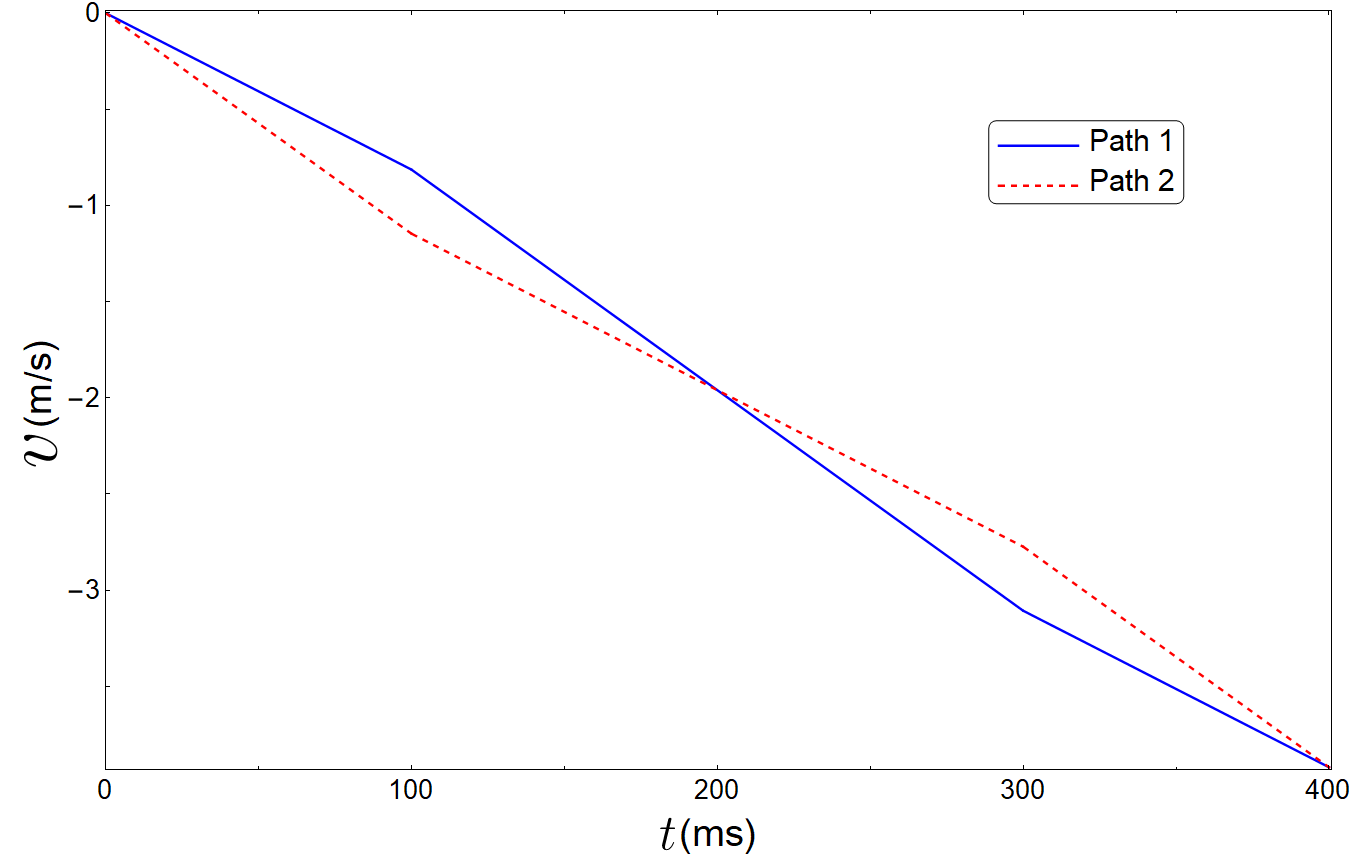
\includegraphics[width=0.8\textwidth]{velocidad.png}
        \caption{Velocity-time graph.}
        \label{velocity_graph}
    \end{subfigure}
    \hfill
    \begin{subfigure}{1\textwidth}
        \centering
        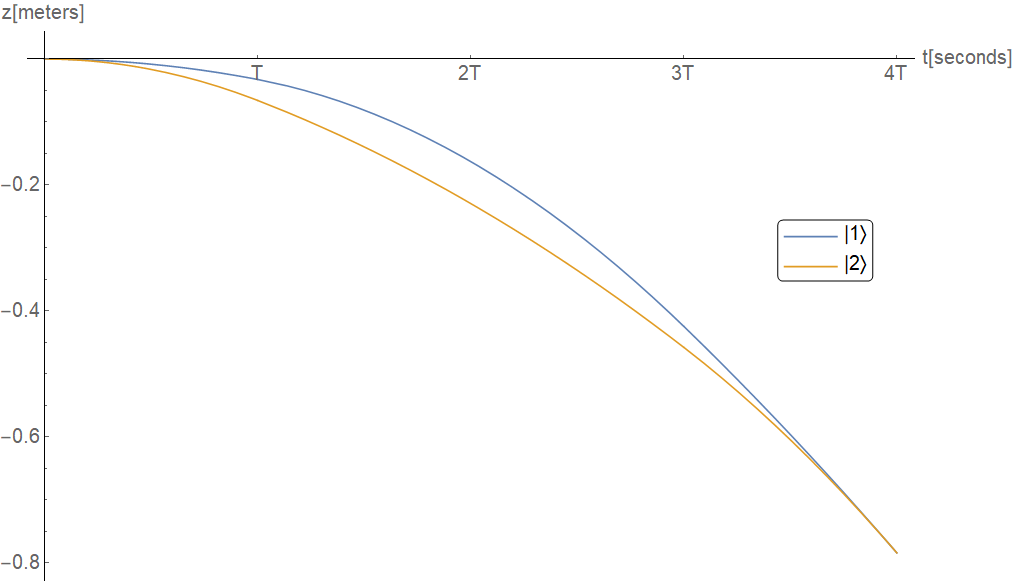
\includegraphics[width=0.8\textwidth]{posicion.png}
        \caption{Position-time graph.}
        \label{position_graph}
    \end{subfigure}
    \caption{Velocity and position vs. time graphs for each state after the superposition of hyperfine levels is created and just before they are made interfere. In these graphs $g=9.8m/s^2$, the mass $m$ is taken to be $87*1.6*10^{-27} Kg$ (approximately the mass of $\ce{^{87}_{}Rb}$), $\mu$ is taken to be the Bohr magneton with value $9.27*10^{-24} J/T$, $\eta$ has a value of $0.05 T/m$, and $T=100ms$. 
    The hyperfine state $\ket{1}$ has a quantum magnetic number of $m_{F}=F$ whereas the state $\ket{2}$ has a value of $m_{F}=-F$.}
    \label{velocity_position_graphs}
\end{figure}

\paragraph{Calculation of the Signal for Gravimetry}
Now that we have settled down the sequence of pulses needed to produce interference, we are in a position to compute the expected signal for gravimetry. In the semi-classical picture, each state of the superposition follows a different path and consequently accumulates a different phase. Therefore, to obtain the gravimetry signal, we need to compute the phase accumulated by each state during the lifetime of the superposition and then compute the difference between these two phases. 

The phase accumulated for each path is given by

\begin{equation}
\Phi = \int_{t_{0}}^{t} \omega(\ce{^{}_{}t{'}_{}})d\ce{^{}_{}t{'}_{}}
\end{equation}

where the angular frequency is given by the Planck relation $\omega = E / \hbar$, and the energy is given by the sum of the magnetic energy (Eq. \ref{magnetic_force}) and the energy due to the gravity field, i.e.,

\begin{equation}\label{classic_energy}
E = \pm \mu B + mgz = (\pm \mu \eta + mg)z = C_{\pm} z
\end{equation}

where we have defined the constant

\begin{equation}\label{c_definition}
C_{\pm} \equiv \pm \mu \eta + mg = m a_{\pm}
\end{equation}

with units of force and with $a_{\pm}$ defined as in the Eqs. \ref{a1} and \ref{a2}. Notice that we have defined the constant $g$ to be positive and we are using a coordinate system with the z-axis pointing upwards such that the atom is initially located at $z=0$, where the initial gravitational potential energy is zero, and as it falls down, the position coordinate becomes negative so the gravitational potential energy becomes negative.

Thus, accumulated phase will be given by

\begin{equation}\label{semi_classical_phase}
\Phi = \frac{C_{\pm}}{\hbar} \int_{t_{0}}^{t} z(\ce{^{}_{}t{'}_{}})d\ce{^{}_{}t{'}_{}}
\end{equation}

Each state's path is composed by three intervals $T_{1}=T$, $T_{2}=2T$, and $T_{3}=T$ (see Eq. \ref{pulses}). Thereby, for the first interval, the phase accumulated by each state will be respectively

\begin{equation}\label{phi1t1}
\Phi_{1, T_{1}} = \frac{C_{-}}{\hbar} \int_{0}^{T} (z_{0}+v_{0}t+a_{+} \frac{t^{2}}{2})dt
\end{equation}

\begin{equation}
\Phi_{2, T_{1}} = \frac{C_{+}}{\hbar} \int_{0}^{T} (z_{0}+v_{0}t+a_{-} \frac{t^{2}}{2})dt
\end{equation}

where $z_{0}$ and $v_{0}$ are respectively the initial position and velocity,
and the accelerations $a_{+}$ and $a_{-}$ are given by Eqs. \ref{a1} and \ref{a2}. The phase difference accumulated during the first interval is

\begin{equation}
\Delta \Phi_{T_{1}} = \Phi_{1, T_{1}} - \Phi_{2, T_{1}}
\end{equation}

Likewise, the phase accumulated during the second interval for each state is

\begin{equation}
\Phi_{1, T_{2}} = \frac{C_{+}}{\hbar} \int_{0}^{2T} [(z_{0}+v_{0}T+a_{+} \frac{T^{2}}{2}) + (v_{0}+a_{+}T)t + a_{-} \frac{t^{2}}{2}]dt
\end{equation}

\begin{equation}
\Phi_{2, T_{2}} = \frac{C_{-}}{\hbar} \int_{0}^{2T} [(z_{0}+v_{0}T+a_{-} \frac{T^{2}}{2}) + (v_{0}+a_{-}T)t + a_{+} \frac{t^{2}}{2}]dt
\end{equation}

The corresponding phase difference for this interval is

\begin{equation}
\Delta \Phi_{T_{2}} = \Phi_{1, T_{2}} - \Phi_{2, T_{2}}
\end{equation}

Finally, for the last interval, the phase accumulated by each state is

\begin{equation}
\Phi_{1, T_{3}} = \frac{C_{-}}{\hbar} \int_{0}^{T} [((z_{0}+v_{0}T+a_{+} \frac{T^{2}}{2}) + (v_{0}+a_{+}T)(2T) + a_{-} \frac{(2T)^{2}}{2}) + (v_{0}+a_{+}T + a_{-}(2T))t + a_{+} \frac{t^{2}}{2}]dt
\end{equation}

\begin{equation}
\Phi_{2, T_{3}} = \frac{C_{+}}{\hbar} \int_{0}^{T} [((z_{0}+v_{0}T+a_{-} \frac{T^{2}}{2}) + (v_{0}+a_{-}T)(2T) + a_{+} \frac{(2T)^{2}}{2}) + (v_{0}+a_{-}T + a_{+}(2T))t + a_{-} \frac{t^{2}}{2}]dt
\end{equation}

The phase difference accumulated during the last interval is

\begin{equation}\label{delphi3}
\Delta \Phi_{T_{3}} = \Phi_{1, T_{3}} - \Phi_{2, T_{3}}
\end{equation}

Therefore, by using Eqs.(\ref{a1}-\ref{a2} , and \ref{phi1t1}-\ref{delphi3}), the total phase difference accumulated during the three intervals is

\begin{equation}
\Delta \Phi = \Delta \Phi_{T_{1}} + \Delta \Phi_{T_{2}} + \Delta \Phi_{T_{3}} = 8 \frac{mga_{m}T^3}{\hbar}
\end{equation}

\begin{equation}\label{gravimetry_signal}
\Delta \Phi = 8 \frac{\mu \eta}{\hbar} g T^3
\end{equation}

where in the last equation we have used the definition of $a_B$ (Eq. \ref{am}). 

The Eq. \ref{gravimetry_signal} is the signal for gravimetry, which is proportional to $T^3$ and also proportional to the magnetic field via the constant $\eta$, these are the parameters we can adjust within a gravimetric experiment in order to increase the precision of the measurement. In Fig.\ref{phase_graph}, we can see the strong of the gravimetry signal for typical values of the constants in Eq. \ref{gravimetry_signal}. 

Finally, we can compare this result with the signal measured in traditional gravimetry that uses stimulated Raman transitions to induce state transitions and changes in momentum \cite{Peters_2001}

\begin{equation}\label{traditional_gravimetry_signal}
\Delta \Phi = k_{eff} g T^2 ,
\end{equation}

where $\hbar k_{eff}$ is the effective momentum gained by the atom after the Raman transition has finished.

\begin{figure}
\centering
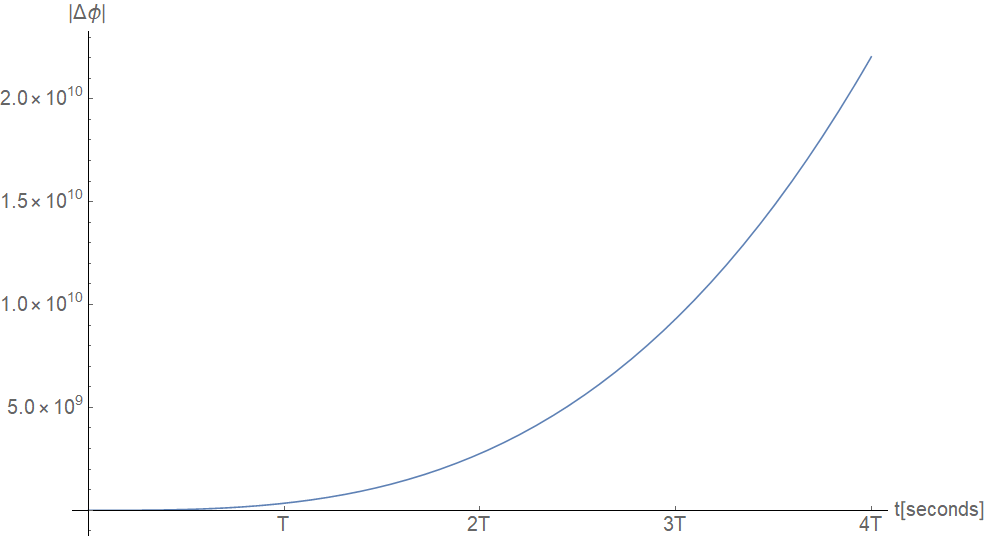
\includegraphics[width=0.9\textwidth]{fase.png}
\caption{Gravimetry signal for an atom falling down inside a linear magnetic field. This graph was obtained by using the same constant values as described in Fig.\ref{velocity_position_graphs}.}
\label{phase_graph}
\end{figure}

\subsubsection{Quantum Picture}
The calculations above were made by using a semi-classical picture to represent the superposition of states. Nevertheless, a correct calculation of the signal for gravimetry demands solving the Schrodinger equation for the evolution of each state in the superposition. 

In the following, we will consider a coherent wave packet of alkali-metal atoms with quantized center-of-mass motion along the z-axis, subject to a constant gravitational field and interacting with a classical magnetic field of the form given by Eq. \ref{magnetic_field}. The wave packet is given at time $t=0$ by

\begin{equation}\label{wave_packet}
\psi(z,0) = 
\left[\frac{1}{2 \pi (\Delta Z(0))^2} \right]^{1/4} \exp \left[-\frac{1}{4} \left[\frac{z-z_{0}}{\Delta Z(0)}\right]^{2}  + i \frac{p_{0}}{\hbar}z \right]
\end{equation}

where $z$ is the position coordinate, $\Delta Z(0)$ is the width of the wave packet centered at $z_{0}$, and $\frac{p_{0}}{\hbar}$ is the wave number of the wave packet. 

Before continuing, we introduce the non-dimensional position $x \equiv \kappa z$, and define the non-dimensional representation of this wave packet as

\begin{equation}\label{wave_packet_non_dimensional}
\phi(x,0) \equiv \frac{1}{\sqrt{\kappa}} \psi(\frac{x}{\kappa}, 0)
\end{equation}

where we have defined the inverse of the characteristic length of the system as

\begin{equation}\label{kappa}
\kappa \equiv (g_{s}\frac{\mu_{B}}{\hbar} + g_{n}\frac{\mu_{n}}{\hbar}) \frac{\eta}{\Delta W} > 0
\end{equation}

where $g_{s}$ is the electron spin $g$ factor, $g_{n}$ is the nuclear $g$ factor, $\mu_{B}$ is the Bohr magneton, $\mu_{n}$ is the nuclear magneton, $\hbar \Delta W$ is the field-free ground-state hyperfine splitting energy, and $\eta$ is the proportionality constant of the magnetic field (Eq. \ref{magnetic_field}).

The time-evolution of the non-dimensional wave packet (Eq. \ref{wave_packet_non_dimensional}) is given by\footnote{The wave packet in the Eq. \ref{wave_packet_non_dimensional_evolution} is already normalized in position for all times.} (see \cite{Castanos2014} for additional details)

\begin{equation}\label{wave_packet_non_dimensional_evolution}
\phi(x,\tau) = 
\left[\frac{1}{2 \pi (\sigma_{x}(\tau))^2} \right]^{1/4} \exp \left[-\frac{1}{4} \left[\frac{x-\xi(\tau)}{\sigma_{x}(\tau)}\right]^{2}  + i\Theta_{p}(x, \tau) - \frac{i}{2}\arctan\left[\frac{\epsilon \tau}{(\sigma_{x}(0))^{2}}\right] \right]
\end{equation}

where $\tau\equiv \Delta W t$ is the non-dimensional time, and we have defined 

\begin{multline}\label{theta_p}
\Theta_{p}(x,\tau) = -\tau \bigg(q_{1} + \frac{\epsilon}{3} q_{2}^{2} \tau^{2}\bigg) + \left[\frac{\sigma_{x}(0)}{\sigma_{x}(\tau)} \right]^{2} (\rho_{0} - q_{2} \tau)(x-\rho_{0} \epsilon \tau) \\
+ \frac{\epsilon \tau}{4 [\sigma_{x}(\tau)\sigma_{x}(0)]^{2}} \left[(x-x_{0})^{2} + 4\rho_{0} x_{0} \epsilon \tau -2q_{2} \epsilon \tau^{2} \bigg(x+x_{0}- \frac{q_{2}}{2} \epsilon \tau^{2} \bigg)\right]
\end{multline}

where we have introduced the following non-dimensional quantities

\begin{equation}\label{non_dimensional_definitions}
\sigma_{x}(0) = \kappa \Delta Z(0)\mathrm{,}\quad \rho_{0}=\frac{p_{0}}{\hbar \kappa} \mathrm{,}\quad 
x_{0}=\kappa z_{0} \mathrm{,}\quad 
\sigma_{x}(\tau) = \sqrt{[\sigma_{x}(0)]^{2} + \left[\frac{\epsilon \tau}{\sigma_{x}(0)} \right]^{2}}
\end{equation}

were $\epsilon$ is given by 

\begin{equation}\label{epsilon}
\epsilon = \frac{\hbar \kappa^{2}}{2 M \Delta W}
\end{equation}

where $M$ is the mass of the atom. Also, we have defined

\begin{equation}\label{q1_q2}
q_{1} = \frac{1}{2} \mathrm{,}\quad q_{2} = \bigg(\frac{M g}{\hbar \Delta W \kappa} \pm  \gamma_{1} \bigg)
\end{equation}

where $g_{0}$ is the acceleration of gravity, and 

\begin{equation}\label{gamma_1}
\gamma_{1} = \frac{g_{s}-2 I g_{n} \frac{m_{e}}{m_{p}}}{2(g_{s}+g_{n}\frac{m_{e}}{m_{p}})}
\end{equation}

where $m_{e}$ and $m_{p}$ are the electron mass and the proton mass respectively, and $I$ is the nuclear spin (assumed to be $I\ \ge 1/2$).
We will see lately when comparing with the time evolution of the free wave packet that $\Delta W q_{1}$ corresponds to the angular frequency and therefore, it is related with the energy of the wave packet.


Additionally, we have defined the following non-dimensional quantity

\begin{equation}\label{xi}
\xi(\tau) = x_{0} + 2 \rho_{0} \epsilon \tau - q_{2}\epsilon \tau^{2}
\end{equation}

The above equation describes the motion of the center of the wave packet with respect to the non-dimensional time $\tau$ as can be seen by using Eqs. \ref{non_dimensional_definitions} and \ref{epsilon} to cast the equation into its dimensional form as follows

\begin{equation}\label{xi_dimensional}
z(t) = \frac{\xi}{\kappa} = z_{0} +  \beta_{0} t +  \frac{\alpha t^{2}}{2}
\end{equation}

where the initial velocity is

\begin{equation}
\beta_{0} = \frac{p_{0}}{M}
\end{equation}

and the acceleration is given by

\begin{equation}\label{q2_a}
\alpha = -q_{2} \frac{ \hbar \kappa \Delta W}{M}
\end{equation}

Therefore, it is convenient to re-write Eq. \ref{xi} as

\begin{equation}\label{xi_eq_motion}
\xi(\tau) = x_{0} + v_{0} \tau + \frac{a \tau^{2}}{2}
\end{equation}

where $v_{0}$ is the non-dimensional initial velocity and $a$ is the non-dimensional acceleration given by

\begin{equation}\label{xi_defs_eq_motion}
v_{0} = 2\rho_{0} \epsilon \mathrm{,}\quad a = -2 q_{2} \epsilon
\end{equation}

Therefore, the non-dimensional velocity of the center of the wave packet will be given by the derivative of Eq. \ref{xi} with respect to $\tau$, i.e.,

\begin{equation}\label{xi_derivative}
\frac{d\xi}{d\tau} = \xi^{\prime}(\tau) =  2 \rho_{0} \epsilon - 2 q_{2}\epsilon \tau = v_{0} + a \tau
\end{equation}

For that reason, Eqs. \ref{xi} and \ref{xi_derivative} are the equations of motion of the center of the (non-dimensional) wave packet. Additionally, we notice that the information about the acceleration of the wave-packet is contained in the parameter $q_{2}$. This parameter is obviously related to the accelerations defined in Eqs. \ref{a1} and \ref{a2} and by consequence with the constant $C_{\pm}$ defined in Eq. \ref{c_definition}.

\paragraph{Calculation of the Signal for Gravimetry in Position Space}

Now, we proceed to compute the signal for gravimetry by using Eq. \ref{wave_packet_non_dimensional_evolution}. In order to do so, we identify the phase of the wave packet

\begin{equation}
\varphi(x, \tau) = \Theta_{p}(x, \tau) - \frac{1}{2}\arctan\left[\frac{\epsilon \tau}{(\sigma_{x}(0))^{2}}\right]
\end{equation}

or more explicitly, using Eq. \ref{theta_p}

\begin{multline}\label{quantum_phase}
\varphi(x, \tau) = -\tau \bigg(q_{1} + \frac{\epsilon}{3} q_{2}^{2} \tau^{2}\bigg) + \left[\frac{\sigma_{x}(0)}{\sigma_{x}(\tau)} \right]^{2} (\rho_{0} - q_{2} \tau)(x-\rho_{0} \epsilon \tau) \\
+ \frac{\epsilon \tau}{4 [\sigma_{x}(\tau)\sigma_{x}(0)]^{2}} \left[(x-x_{0})^{2} + 4\rho_{0} x_{0} \epsilon \tau -2q_{2} \epsilon \tau^{2} \bigg(x+x_{0}- \frac{q_{2}}{2} \epsilon \tau^{2} \bigg)\right] 
- \frac{1}{2}\arctan\left[\frac{\epsilon \tau}{(\sigma_{x}(0))^{2}}\right]
\end{multline}

The above equation contains several corrections to the phase computed by using Eq. \ref{semi_classical_phase} which was obtained by using a semi-classical approach. The last term in Eq. \ref{quantum_phase} does not contribute to the phase difference, as we will see in the next section\footnote{The last term does not have any dependence on the initial velocity, initial position, and/or $q_{2}$, therefore, its contribution to the phase difference will be zero.}, and we can ignore it. The semi-classical result (Eq. \ref{gravimetry_signal}) can be reproduced by using the following approximation

\begin{equation}\label{sigma_zero_approx}
\sigma_{x}(0) \gg \epsilon \tau,
\end{equation}

in the definition of $\sigma_{x}(\tau)$ which we rewrite here

\begin{equation*}
\sigma_{x}(\tau) = \sqrt{[\sigma_{x}(0)]^{2} + \left[\frac{\epsilon \tau}{\sigma_{x}(0)} \right]^{2}},
\end{equation*}

therefore, using this approximation we can write

\begin{equation*}
\sigma_{x}(\tau) \approx \sigma_{x}(0),
\end{equation*}

so we will have the following

\begin{equation}\label{sigma_quotient_approx}
\left[\frac{\sigma_{x}(0)}{\sigma_{x}(\tau)} \right]^{2} \approx 1 \mathrm{,}\quad \frac{\epsilon \tau}{ [\sigma_{x}(\tau)\sigma_{x}(0)]^{2}} \approx 0.
\end{equation}

The physical interpretation of this approximation (Eq. \ref{sigma_zero_approx}) is that the widening of the wave packet during the experiment is negligible. In other words, the waist of the wave packet remains approximately constant.

Therefore, using the approximation in Eq. \ref{sigma_zero_approx} (and discarding the term that does not contribute at all) allows us to approximate the phase (Eq. \ref{quantum_phase}) as

\begin{equation}\label{approx_quantum_phase}
\varphi_{\pm}(x, \tau) \approx -\tau \bigg(q_{1} + \frac{\epsilon}{3} q_{2_{\pm}}^{2} \tau^{2}\bigg) + (\rho_{0} - q_{2_{\pm}} \tau)(x-\rho_{0} \epsilon \tau)
\end{equation}

where we have used a sub-index to indicate whether we are considering $q_{2}$ with the plus or minus sign in front of the constant $\gamma_{1}$. 

Before diving deep into the computation of the phase difference, let's analyze the above equation. The second term is the product of two differences. The first term is 

\begin{equation}\label{momentum_change}
(\rho_{0} - q_{2_{\pm}} \tau),
\end{equation}

according to Eq. \ref{non_dimensional_definitions}, this term accounts for the increase in momentum of the wave-packet, therefore, it can be interpreted as the difference between the initial momentum $\rho_{0}$ and the final momentum $q_{2_{\pm}} \tau$ acquired due to the acceleration. In the same way, the second term is

\begin{equation}\label{position_change}
(x-\rho_{0} \epsilon \tau),
\end{equation}

according to Eq. \ref{xi_defs_eq_motion}, the product $\rho_{0} \epsilon$ represents the initial velocity of the wave packet, therefore, the above term represents the difference between the non-dimensional position $x$ and half of the non-dimensional distance acquired due to the initial velocity of the wave packet.

Now, we are in position to compute the signal for gravimetry using Eq. \ref{approx_quantum_phase}, and the sequence of pulses shown in Eq. \ref{pulses}. Also, according to Eq. \ref{approx_quantum_phase}, the phase obtained will depend on the non-dimensional position $x$, thereby, all the contributions to the phase have to be computed with respect to the same $x$ which we will call\footnote{$x_{d}$ can be, for instance, the position of the detector at the end of the experiment.} $x_{d}$.

Let's analyze the first interval. The initial momentum and velocity of the wave packet are respectively $\rho_{0}$ and $v_{0}$. Thereby, the phase acquired during the first interval will be

\begin{equation}\label{approx_quantum_phase_1}
\varphi_{\pm, \tau_{1}}(x) \approx -\tau \bigg(q_{1} + \frac{\epsilon}{3} q_{2_{\pm}}^{2} \tau^{2}\bigg) + (\rho_{0} - q_{2_{\pm}} \tau)(x-\frac{v_{0} \tau}{2})
\end{equation}

where we have used the definition of $v_{0}$, Eq. \ref{xi_defs_eq_motion}.
For the second interval (with period $2\tau$), the initial momentum of the wave-packet will be $(\rho_{0} - q_{2_{\pm}} \tau)$ and the initial velocity will be $(v_{0}+a_{\pm}\tau)$, where the acceleration $a_{\pm}$ was defined in Eq. \ref{xi_defs_eq_motion} and the sub-index indicates the sign used in $q_{2}$ (Eq. \ref{q1_q2}). Therefore, the phase accumulated during the second interval will be given by

\begin{equation}\label{approx_quantum_phase_2}
\varphi_{\pm, \tau_{2}}(x) \approx -(2\tau) \bigg(q_{1} + \frac{\epsilon}{3} q_{2_{\mp}}^{2} (2\tau)^{2}\bigg) + ((\rho_{0} - q_{2_{\pm}} \tau)-q_{2_{\mp}} (2\tau))(x-\frac{(v_{0}+a_{\pm}\tau) (2\tau)}{2})
\end{equation}

where we have used a sub-index in $a$ to indicate the sign of $\gamma_{1}$ in the definition of $q_{2}$.
Similarly, the initial momentum of the wave-packet for the third interval will be $(\rho_{0} - q_{2_{\pm}} \tau-2q_{2_{\mp}}\tau)$ and the initial velocity will be $(v_{0}+a_{\pm}\tau + 2 a_{\mp}\tau)$, thus the phase acquired during this interval will be given by

\begin{equation}\label{approx_quantum_phase_3}
\varphi_{\pm, \tau_{3}}(x) \approx -\tau \bigg(q_{1} + \frac{\epsilon}{3} q_{2_{\pm}}^{2} \tau^{2}\bigg) + ((\rho_{0} - q_{2_{\pm}} \tau-2q_{2_{\mp}}\tau)-q_{2_{\pm}} \tau)(x-\frac{(v_{0}+a_{\pm}\tau + 2a_{\mp}\tau) \tau}{2})
\end{equation}

Therefore, the phase difference accumulated during the first interval, and evaluated at the position $x_{d}$ will be given by

\begin{equation}
\Delta \Phi_{\tau_{1}}(x_{d}) = \varphi_{+,\tau_{1}}(x_{d}) - \varphi_{-,\tau_{1}}(x_{d})
\end{equation}

whereas for the second interval, evaluated at $x_{d}$, we have

\begin{equation}
\Delta \Phi_{\tau_{2}}(x_{d}) = \varphi_{-,\tau_{2}}(x_{d}) - \varphi_{+,\tau_{2}}(x_{d})
\end{equation}

and finally, for the last interval, evaluated at $x_{d}$, we have

\begin{equation}
\Delta \Phi_{\tau_{3}}(x_{d}) = \varphi_{+,\tau_{3}}(x_{d}) - \varphi_{-,\tau_{3}}(x_{d})
\end{equation}

Thereby, the total phase difference accumulated during the three intervals at $x_{d}$ is given by 

\begin{equation}\label{pre_total_quantum_phase}
\Delta \Phi (x_{d}) = \Delta \Phi_{\tau_{1}}(x_{d}) + \Delta \Phi_{\tau_{2}}(x_{d}) + \Delta \Phi_{\tau_{3}}(x_{d})
\end{equation}

Now, before substituting numerical values, we will make additional approximations. Firstly, we need an approximation for $\kappa$ defined in Eq. \ref{kappa}. The Bohr magneton, and the nuclear magneton are defined as

\begin{equation}
\mu_{B} = \frac{\hbar e}{2 m_{e}} \mathrm{,}\quad \mu_{n} = \frac{\hbar e}{2 m_{p}}
\end{equation}

where $m_{e}$ and $m_{p}$ are the electron and proton mass respectively. However, the proton mass is several orders of magnitude larger than the electron mass, therefore, we can use the following approximation

\begin{equation}\label{kappa_approx}
\kappa \approx g_{s}\frac{\mu }{\hbar} \frac{\eta}{\Delta W}
\end{equation}

where we have used the approximation $\mu_{B} \approx \mu$, where $\mu$ is the total magnetic moment of the atom. Additionally, by considering the alkali atoms to be $\ce{^{87}_{}Rb}$ atoms. We have the following values for this atom \cite{KAUSHALSK1970,Bunge1993}

\begin{equation}
g_{s} \approx 2.002 \mathrm{,}\quad g_{n} \frac{m_{e}}{m_{p}} \approx 2.002 \mathrm{,}\quad I = \frac{3}{2}
\end{equation}

thereby, we can approximate $\gamma_{1}$ defined in Eq. \ref{gamma_1} as

\begin{equation}\label{gamma_1_approx}
\gamma_{1} \approx 1/2
\end{equation}

Finally, by using Eqs.(\ref{approx_quantum_phase_1}-\ref{pre_total_quantum_phase}), the definitions Eqs.(\ref{non_dimensional_definitions}-\ref{gamma_1}) alongside the approximations in Eqs. \ref{kappa_approx}, \ref{gamma_1_approx}, we obtain

\begin{equation}
\Delta \Phi_{\tau_{1}}(x_{d}) = -x_{d}\tau + \frac{\eta \mu \tau^{2} p_{0}}{M \hbar \Delta W^{2}} - \frac{2 \eta \mu \tau^{3} g}{3 \hbar \Delta W^{3}}
\end{equation}

\begin{equation}
\Delta \Phi_{\tau_{2}}(x_{d}) = x_{d}\tau + \frac{4 \eta \mu \tau^{3} g}{3 \hbar \Delta W^{3}}
\end{equation}

\begin{equation}
\Delta \Phi_{\tau_{3}}(x_{d}) = -\frac{\eta \mu \tau^{2} p_{0}}{M \hbar \Delta W^{2}} + \frac{10 \eta \mu \tau^{3} g}{3 \hbar \Delta W^{3}}
\end{equation}

\begin{equation}\label{quantum_gravimetry_signal}
\Delta \Phi = 4 \frac{\mu \eta }{\hbar} g \bigg(\frac{\tau}{\Delta W}\bigg)^{3} = 4 \frac{\mu \eta }{\hbar} g t^{3},
\end{equation}

were we have used the definition of the non-dimensional time ($\tau\equiv \Delta W t$). Thus, we see that in the quantum picture, the total phase difference is half the phase difference obtained in the semi-classical computation Eq. \ref{gravimetry_signal}. In addition, it can be seen that the total phase difference does not depend on the position $x_{d}$ as expected.

\paragraph{First-Order Correction to the Gravimetry Signal}
In this section, we will analyze the contribution of the rest of the terms in Eq. \ref{quantum_phase}, which we re-write here

\begin{multline*}\label{quantum_phase_revisited}
\varphi(x, \tau) = -\tau \bigg(q_{1} + \frac{\epsilon}{3} q_{2}^{2} \tau^{2}\bigg) + \left[\frac{\sigma_{x}(0)}{\sigma_{x}(\tau)} \right]^{2} (\rho_{0} - q_{2} \tau)(x-\rho_{0} \epsilon \tau) \\
+ \frac{\epsilon \tau}{4 [\sigma_{x}(\tau)\sigma_{x}(0)]^{2}} \left[(x-x_{0})^{2} + 4\rho_{0} x_{0} \epsilon \tau -2q_{2} \epsilon \tau^{2} \bigg(x+x_{0}- \frac{q_{2}}{2} \epsilon \tau^{2} \bigg)\right] 
- \frac{1}{2}\arctan\left[\frac{\epsilon \tau}{(\sigma_{x}(0))^{2}}\right]
\end{multline*}.

In the computation of the last section, we ignored the following terms

\begin{equation*}
\frac{\epsilon \tau}{4 [\sigma_{x}(\tau)\sigma_{x}(0)]^{2}} \left[(x-x_{0})^{2} + 4\rho_{0} x_{0} \epsilon \tau -2q_{2} \epsilon \tau^{2} \bigg(x+x_{0}- \frac{q_{2}}{2} \epsilon \tau^{2} \bigg)\right] 
- \frac{1}{2}\arctan\left[\frac{\epsilon \tau}{(\sigma_{x}(0))^{2}}\right]
\end{equation*}

We want to know what is the contribution of these terms to the total phase difference and get a correction for the result obtained in Eq. \ref{quantum_gravimetry_signal}. Let us begin using Eq. \ref{xi_defs_eq_motion} to re-write the above terms as 

\begin{equation}\label{quantum_phase_ignored_terms}
\frac{\epsilon \tau}{4 [\sigma_{x}(\tau)\sigma_{x}(0)]^{2}} \left[(x-x_{0})^{2} + 2v_{0} x_{0} \tau +a \tau^{2} \bigg(x+x_{0}+ \frac{a}{4} \tau^{2} \bigg)\right] 
- \frac{1}{2}\arctan\left[\frac{\epsilon \tau}{(\sigma_{x}(0))^{2}}\right]
\end{equation}

We can notice in the above equation that the last term does not have any dependence on the initial conditions (position and/or velocity) nor the acceleration. Therefore, since the initial conditions will have a dependence on $a$ (and consequently a dependence on $q_{2}$) for the second and third intervals, the contribution of the last term to the final phase difference will be trivially zero. Then, we can safely ignore the last term since its contribution will be zero and only consider the following terms:

\begin{equation}\label{quantum_phase_ignored_terms_simplified}
\frac{\epsilon \tau}{4 [\sigma_{x}(\tau)\sigma_{x}(0)]^{2}} \left[(x-x_{0})^{2} + 2v_{0} x_{0} \tau +a \tau^{2} \bigg(x+x_{0}+ \frac{a}{4} \tau^{2} \bigg)\right].
\end{equation}

Now, we can expand the first term inside the square brackets and use the same argument as before to ignore the $x^{2}$ term. Thereby, it only remains to study the contribution to the signal of the following terms

\begin{equation}\label{quantum_phase_ignored_terms_simplified_expanded}
\frac{\epsilon \tau}{4 [\sigma_{x}(\tau)\sigma_{x}(0)]^{2}} \left[-2x x_{0}+x_{0}^{2} + 2v_{0} x_{0} \tau +a \tau^{2} \bigg(x+x_{0}+ \frac{a}{4} \tau^{2} \bigg)\right].
\end{equation}

The contribution of these terms to the final signal is not trivial. We will study its contribution to the final result using the Eq. \ref{quantum_phase_ignored_terms_simplified}  because it is easier to manipulate. We will repeat the computation of the last section, however, this time, we will not use the approximation in Eq. \ref{sigma_zero_approx} Therefore, at the end of the first interval, the phase will be given by

\begin{multline}\label{quantum_phase_ignored_terms_simplified_t1}
\varphi_{\pm, \tau_{1}}(x) =-\tau \bigg(q_{1} + \frac{\epsilon}{3} q_{2_{\pm}}^{2} \tau^{2}\bigg) + \bigg[\frac{\sigma_{x, \tau_{0}}}{\sigma_{x, \tau_{1}}}\bigg]^{2}(\rho_{0} - q_{2_{\pm}} \tau)(x-\frac{v_{0} \tau}{2}) \\
+ \frac{\epsilon \tau}{4 [\sigma_{x, \tau_{1}}\sigma_{x, \tau_{0}}]^{2}} \left[(x-x_{0})^{2} + 2v_{0} x_{0} \tau +a_{\pm} \tau^{2} \bigg(x+x_{0}+ \frac{a_{\pm}}{4} \tau^{2} \bigg)\right],
\end{multline}

where we have used, as usual, a sub-index in $a$ to indicate the sign used in the definition of $q_{2}$, and the non-dimensional standard deviation $\sigma_{x, \tau_{1}}$ is given by 

\begin{equation}\label{sigma_x_t1}
\sigma_{x, \tau_{1}} = \sqrt{[\sigma_{x, \tau_{0}}]^{2} + \left[\frac{\epsilon \tau}{\sigma_{x, \tau_{0}}} \right]^{2}},
\end{equation}

where $\sigma_{x, \tau_{0}}$ is the initial standard deviation of the wave-packet.

For the second interval, the initial conditions will have changed such that the phase will be given by

\begin{multline}\label{quantum_phase_ignored_terms_simplified_t2}
\varphi_{\pm, \tau_{2}}(x) = -(2\tau) \bigg(q_{1} + \frac{\epsilon}{3} q_{2_{\mp}}^{2} (2\tau)^{2}\bigg) + \bigg[\frac{\sigma_{x, \tau_{1}}}{\sigma_{x, \tau_{2}}}\bigg]^{2}((\rho_{0} - q_{2_{\pm}} \tau)-q_{2_{\mp}} (2\tau))(x-\frac{(v_{0}+a_{\pm}\tau) (2\tau)}{2})\\ 
+\frac{\epsilon (2\tau)}{4 [\sigma_{x, \tau_{2}}\sigma_{x, \tau_{1}}]^{2}} \bigg[\bigg(x-(x_{0}+v_{0} \tau + \frac{a_{\pm}\tau^{2}}{2})\bigg)^{2}
+ 2(v_{0} + a_{\pm} \tau) (x_{0}+v_{0} \tau + \frac{a_{\pm}\tau^{2}}{2}) (2\tau) \\ 
+a_{\mp} (2\tau)^{2} \bigg(x+(x_{0}+v_{0} \tau + \frac{a_{\pm}\tau^{2}}{2})+ \frac{a_{\mp}}{4} (2\tau)^{2} \bigg)\bigg],
\end{multline}

where the new standard deviation $\sigma_{x, \tau_{2}}$ will be given in terms of the new initial standard deviation $\sigma_{x, \tau_{1}}$ as follows

\begin{equation}\label{sigma_x_t2}
\sigma_{x, \tau_{2}} = \sqrt{[\sigma_{x, \tau_{1}}]^{2} + \left[\frac{\epsilon (2\tau)}{\sigma_{x, \tau_{1}}} \right]^{2}}
\end{equation}

Similarly, for the last interval we will have

\begin{multline}\label{quantum_phase_ignored_terms_simplified_t3}
\varphi_{\pm, \tau_{3}}(x) = -\tau \bigg(q_{1} + \frac{\epsilon}{3} q_{2_{\pm}}^{2} \tau^{2}\bigg) + \bigg[\frac{\sigma_{x, \tau_{2}}}{\sigma_{x, \tau_{3}}}\bigg]^{2}((\rho_{0} - q_{2_{\pm}} \tau-2q_{2_{\mp}}\tau)-q_{2_{\pm}} \tau)(x-\frac{(v_{0}+a_{\pm}\tau + 2a_{\mp}\tau) \tau}{2}) \\
+ \frac{\epsilon \tau}{4 [\sigma_{x, \tau_{3}}\sigma_{x, \tau_{3}}]^{2}} \bigg[\bigg(x-\Big((x_{0}+v_{0} \tau + \frac{a_{\pm}\tau^{2}}{2}) + (v_{0}+a_{\pm}\tau)(2\tau) + \frac{a_{\mp}(2\tau)^{2}}{2}\Big)\bigg)^{2}\\
+ 2\bigg(v_{0} + a_{\pm} \tau + 2a_{\mp} \tau\bigg)\bigg((x_{0}+v_{0} \tau + \frac{a_{\pm}\tau^{2}}{2}) + (v_{0}+a_{\pm}\tau)(2\tau) + \frac{a_{\mp}(2\tau)^{2}}{2}\bigg) \tau\\
+a_{\pm} \tau^{2} \bigg(x+\Big((x_{0}+v_{0} \tau + \frac{a_{\pm}\tau^{2}}{2}) + (v_{0}+a_{\pm}\tau)(2\tau) + \frac{a_{\mp}(2\tau)^{2}}{2}\Big)+ \frac{a_{\pm}}{4} \tau^{2} \bigg)\bigg],
\end{multline}

where the new standard deviation $\sigma_{x, \tau_{3}}$ will be given by 

\begin{equation}\label{sigma_x_t3}
\sigma_{x, \tau_{3}} = \sqrt{[\sigma_{x, \tau_{2}}]^{2} + \left[\frac{\epsilon \tau}{\sigma_{x, \tau_{2}}} \right]^{2}}.
\end{equation}

Before proceeding with the computation of the correction for the gravimetry signal, we will give an interpretation of the approximation used in the last section. In order to do so, we need to write the square inverse of $\sigma_{x}(\tau)$ as follows

\begin{equation}\label{sigma_x_beta}
[\sigma_{x}(\tau)]^{-2} = [\sigma_{x}(0)]^{-2}\left[1 + \beta^{2}\right]^{-1},
\end{equation}

where we have defined the parameter $\beta$ as follows

\begin{equation}\label{beta_parameter}
\beta \equiv \frac{\epsilon \tau}{[\sigma_{x}(0)]^{2}}.
\end{equation}

By using a Maclaurin expansion for Eq. \ref{sigma_x_beta} in terms of $\beta$, we can see that the approximation used in the last section (Eq. \ref{sigma_zero_approx}) was just the zeroth-order expansion of $1/\sigma_{x}(\tau)$ in powers of $\beta$, i.e.,

\begin{equation}
\sigma_{x}(\tau) \approx \sigma_{x}(0).
\end{equation}

This approximation means that the width of the wave packet remains constant and is independent of the time. Thus, the width of the wave packet will be the same during all the intervals. i.e., 

\begin{equation}
\sigma_{x, \tau_{0}} \approx \sigma_{x, \tau_{1}} \approx \sigma_{x, \tau_{2}} \approx \sigma_{x, \tau_{3}} 
\end{equation}

Thereby, the approximation in the last section (Eq. \ref{quantum_gravimetry_signal}) was obtained using the zeroth-order approximation of Eq. \ref{sigma_x_beta}.
\vfill

Now, we return to the computation of correction of the gravimetry signal. At the beginning of the experiment, the initial width of the wave packet is given by $\sigma_{x, \tau_{0}}$. The next correction to the zeroth-order approximation is obtained using the first-order expansion of $\beta$. Thus we can consider the final width (Eq. \ref{sigma_x_t1}) to be given at first-order by

\begin{equation}\label{sigma_x_t1_first_order}
[\sigma_{x, \tau_{1}}]^{-2} \approx [\sigma_{x, \tau_{0}}]^{-2}\left[1 - \bigg(\frac{\epsilon \tau}{[\sigma_{x}(0)]^{2}}\bigg)^{2}\right] = [\sigma_{x, \tau_{0}}]^{-2}\left[1 - \beta^{2}\right],
\end{equation}

Likewise, for the second interval, the final width (Eq.  \ref{sigma_x_t2}) will be given at first-order by

\begin{equation}\label{sigma_x_t2_first_order}
[\sigma_{x, \tau_{2}}]^{-2} \approx [\sigma_{x, \tau_{0}}]^{-2}\left[1 - \bigg(\frac{\epsilon (\tau+2\tau)}{[\sigma_{x}(0)]^{2}}\bigg)^{2}\right] = [\sigma_{x, \tau_{0}}]^{-2}\left[1 - 9\beta^{2}\right],
\end{equation}

In the same way, the width at the end of the third interval (Eq. \ref{sigma_x_t3}) will be given at first-order by 

\begin{equation}\label{sigma_x_t3_first_order}
[\sigma_{x, \tau_{3}}]^{-2} \approx [\sigma_{x, \tau_{0}}]^{-2}\left[1 - \bigg(\frac{\epsilon (\tau+2\tau+\tau)}{[\sigma_{x}(0)]^{2}}\bigg)^{2}\right] = [\sigma_{x, \tau_{0}}]^{-2}\left[1 - 16\beta^{2}\right].
\end{equation}

Finally, by using Eqs. \ref{quantum_phase_ignored_terms_simplified_t1}, \ref{quantum_phase_ignored_terms_simplified_t2}, and \ref{quantum_phase_ignored_terms_simplified_t3} alongside the first-order approximations for the width of the wave packet (Eqs. \ref{sigma_x_t1_first_order}, \ref{sigma_x_t2_first_order}, and \ref{sigma_x_t3_first_order}), we can get the total phase difference accumulated by the wave packet in the first-order approximation

\begin{comment}
\begin{multline}
\Delta \Phi = \frac{\tau }{12 \left(1 -10 \beta ^2 + 9 \beta ^4\right)} 
\Bigg[ 24 \tau ^2 \epsilon \text{} \left( \text{$(q_{2_{+}})$}^2- \text{$(q_{2_{-}})$}^2\right) \\
+ \beta ^2 \bigg(6 \left(5 x+3 x_0\right) (\text{$q_{2_{-}}$}-\text{$q_{2_{+}}$})+12 \rho _0 \tau  \epsilon  (\text{$q_{2_{-}}$}-\text{$q_{2_{+}}$}) + 231\tau ^2 \epsilon  \text{} \left( \text{$(q_{2_{-}})$}^2- \text{$(q_{2_{+}})$}^2\right)\bigg) \\
+ \beta ^4 \bigg(6 \left(65 x-51 x_0\right) (\text{$q_{2_{-}}$}-\text{$q_{2_{+}}$})-1896 \rho _0 \tau  \epsilon  (\text{$q_{2_{-}}$}-\text{$q_{2_{+}}$}) + 1377 \tau ^2 \epsilon   \text{} \left( \text{$(q_{2_{-}})$}^2- \text{$(q_{2_{+}})$}^2\right) \bigg) \\
+ \beta ^6 \bigg(18 \left(85 x_0-393 x\right) (\text{$q_{2_{-}}$}-\text{$q_{2_{+}}$})+13440 \rho _0 \tau  \epsilon  (\text{$q_{2_{-}}$}-\text{$q_{2_{+}}$}) -4773 \tau ^2 \epsilon  \left(\text{$(q_{2_{-}})$}^2-\text{$(q_{2_{+}})$}^2\right)\bigg) \\
+ \beta ^8 \bigg(54 \left(199 x-41 x_0\right) (\text{$q_{2_{-}}$}-\text{$q_{2_{+}}$})-32940 \rho _0 \tau  \epsilon  (\text{$q_{2_{-}}$}-\text{$q_{2_{+}}$}) + 32427 \tau ^2 \epsilon  \left(\text{$(q_{2_{-}})$}^2-\text{$(q_{2_{+}})$}^2\right)\bigg) \\
+ \beta ^{10} \bigg(-972 \left(5 x-x_0\right) (\text{$q_{2_{-}}$}-\text{$q_{2_{+}}$})+21384 \rho _0 \tau  \epsilon  (\text{$q_{2_{-}}$}-\text{$q_{2_{+}}$}) -27702 \tau ^2 \epsilon  \left(\text{$(q_{2_{-}})$}^2-\text{$(q_{2_{+}})$}^2\right)\bigg)\Bigg]
\end{multline}
\end{comment}

\begin{multline}
\Delta \Phi = \frac{\tau }{4 \left(1 -10 \beta ^2 + 9 \beta ^4\right)} 
\Bigg[ 8 \tau ^2 \epsilon \text{} \left( \text{$(q_{2_{+}})$}^2- \text{$(q_{2_{-}})$}^2\right) \\
+ \beta ^2 (\text{$q_{2_{-}}$}-\text{$q_{2_{+}}$}) \bigg(2 \left(5 x+3 x_0\right) +4 \rho _0 \tau  \epsilon + 77\tau ^2 \epsilon  \text{} (\text{$q_{2_{-}}$}+\text{$q_{2_{+}}$})\bigg) 
+ \mathcal{O}(\beta ^4) \Bigg].
\end{multline}

This result can be re-written using the definitions \ref{non_dimensional_definitions}-\ref{gamma_1} alongside the approximations \ref{kappa_approx}-\ref{gamma_1_approx} and keeping only quadratic terms in $\beta$ in the denominator as

\begin{equation}
\Delta \Phi = \frac{1}{\left(1 -10 \beta ^2 + 9 \beta ^4\right)} \frac{\mu \eta}{\hbar}
\Bigg[ 4 g t^3
- \beta ^2 \bigg(\frac{77 g t^3}{2} + \frac{p_{0}t^2}{M}  + (3z_{0}+5z)t \bigg) \Bigg],
\end{equation}

where $\beta$ was defined in Eq. \ref{beta_parameter}.
These previous results can be cast into a more illuminating form by expanding the denominator in the first term  and keeping only quadratic terms in $\beta$ as follows

\begin{equation}\label{gravimetry_signal_first_order_approx}
\Delta \Phi ^{(1)} = 
 2 \tau ^3 \epsilon \text{} \left( \text{$(q_{2_{+}})$}^2- \text{$(q_{2_{-}})$}^2\right)
- \beta ^2 \bigg[ \frac{\tau }{4} (\text{$q_{2_{+}}$}-\text{$q_{2_{-}}$}) \left(2 \left(5 x+3 x_0\right) +4 \rho _0 \tau  \epsilon - 3\tau ^2 \epsilon  \text{} (\text{$q_{2_{+}}$}+\text{$q_{2_{-}}$}) \right) \bigg],
\end{equation}

\begin{equation}\label{gravimetry_signal_first_order_approx_dimensional}
\Delta \Phi ^{(1)} =  \frac{\mu \eta}{\hbar}
\Bigg[ 4 g t^3
- \beta ^2 \bigg(-\frac{3 g t^3}{2} + \frac{p_{0}t^2}{M}  + (3z_{0}+5z)t \bigg) \Bigg],
\end{equation}

where we have used a super-index to indicate that these results correspond to the first-order correction.
The comparison between the zeroth-order approximation and the first-order correction can be seen in Fig. \ref{phase_graph_first_order}.

The correction given by the first-order approximation goes like $\beta ^2$. Therefore, the error made by considering the first-order approximation will be set by $\beta ^2$ which for the case of typical experimental values (see description of Fig. \ref{phase_graph_first_order}), has a value of $\beta ^2 \approx 3.3 \times 10^{-10}$. As we can see in the Fig. \ref{fig:gravimetry_signal_zeroth_order}, this gravimetry signal could allow us to measure $g$ with $9$ digits of precision, however, according to the Fig. \ref{fig:gravimetry_signal_first_minus_zeroth_order} the error due to the first-order correction would start affecting the eighth digit of the measurement. Therefore, in reality, we should be able to measure $g$ with $8$ digits of precision. This precision is affected principally by the initial width of the wave packet as can be seen in the definition \ref{beta_parameter}. For every order of magnitude that we increase(decrease) the initial width of the wave packet, we gain(lose) $4$ digits of precision in the measurement because the correction goes like $\beta ^2$.

\begin{figure}
     \centering
     \begin{subfigure}[b]{0.9\textwidth}
         \centering
         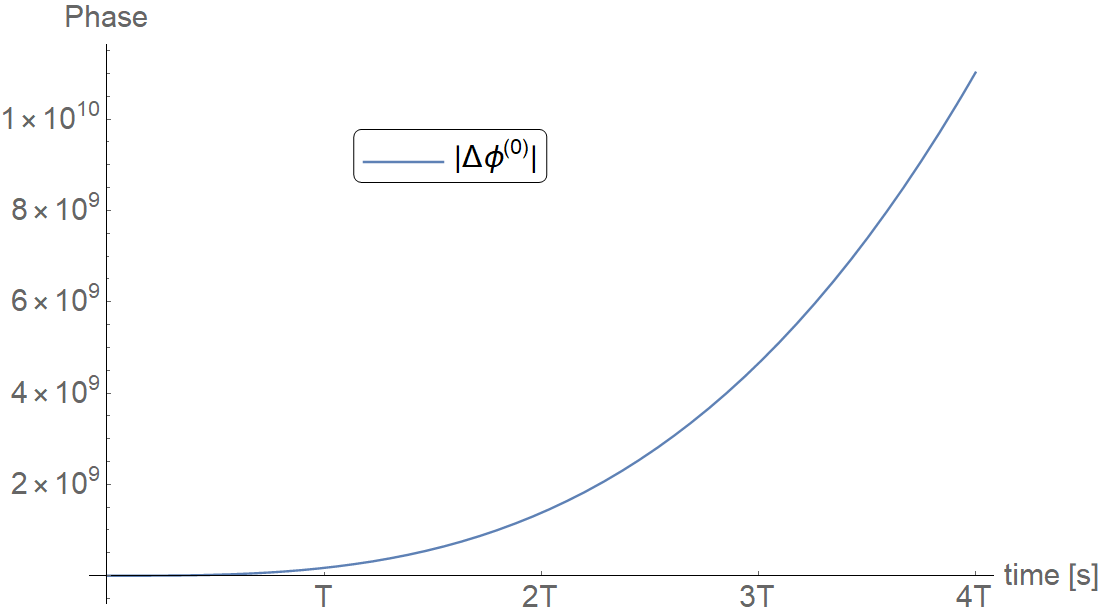
\includegraphics[width=\textwidth]{fase0order.png}
         \caption{Gravimetry signal in the zeroth-order approximation ($\Delta \Phi ^{(0)}$).}
         \label{fig:gravimetry_signal_zeroth_order}
     \end{subfigure}
     \hfill
     \begin{subfigure}[b]{0.9\textwidth}
         \centering
         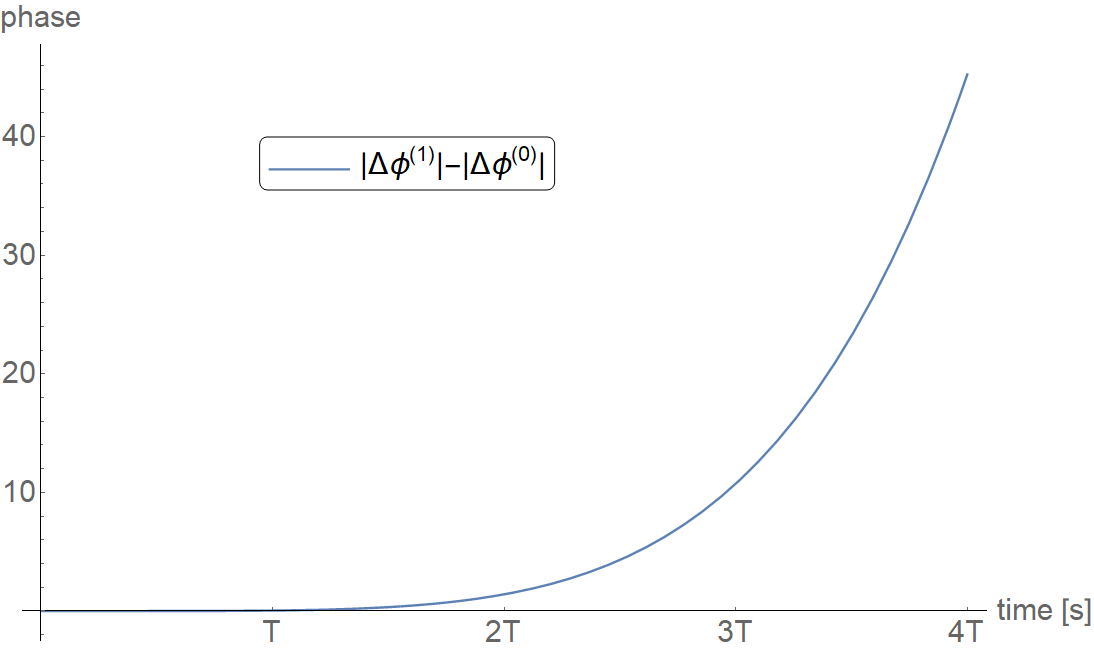
\includegraphics[width=\textwidth]{phase0orderminus1order.png}
         \caption{Phase difference between the zeroth-order approximation ($\Delta \Phi ^{(0)}$) and the first-order approximation ($\Delta \Phi ^{(1)}$), i.e., this is the graph of the correction term (second term) in the Eq. \ref{gravimetry_signal_first_order_approx_dimensional}.}
         \label{fig:gravimetry_signal_first_minus_zeroth_order}
     \end{subfigure}
     \hfill
     \caption{Comparison of the gravimetry signal obtained by using the zeroth-order approximation ($\Delta \Phi ^{(0)}$) given by Eq. \ref{quantum_gravimetry_signal} versus the first-order correction ($\Delta \Phi ^{(1)}$) given by Eq. \ref{gravimetry_signal_first_order_approx_dimensional}. The period used to produce these graphs was $T=50ms$. Besides, we used $g=9.8m/s^{2}$, $\mu=9.27\times10^{-24} J/T$ (the Bohr magneton), $\eta=0.05 T/m$. Additionally, we consider $\ce{^{87}_{}Rb}$ atoms, so we have (\cite{Bunge1993}\cite{KAUSHALSK1970}) $M=1.45\times10^{-25}kg$, $\Delta W=2\pi\times6.835\times10^{9}s^{-1}$ ($\hbar \Delta W $ is the field-free ground state hyperfine energy splitting). Also, we use the approximations in Eqs. \ref{kappa_approx} and \ref{gamma_1_approx}. In addition, we take $p_{0}=0$, $z_{0}=0$, $\Delta Z(0)=1000\times10^{-6}m$, and take $z$ to be the final position of the center of the wave packet at the end of the experiment. The center of the wave packet was evaluated by using the Eq. \ref{xi_eq_motion}, where $x=\kappa z$. In this case, $(\sigma_{x, \tau_{0}})^{2} \approx 4.1 \times 10^{-8}$ and $\epsilon \tau \approx 1.5 \times 10^{-11} t$. Thus, for $t=50ms$, we have $\beta \approx 1.8 \times 10^{-5}$ and the expansion used in the Eqs. \ref{sigma_x_t1_first_order}-\ref{sigma_x_t3_first_order} is justified. Moreover, the gap between both approximations will be proportional to $\beta ^2 \approx 3.3 \times 10^{-10}$.}
     \label{phase_graph_first_order}
\end{figure}


\paragraph{Calculation of the Signal for Gravimetry in Momentum Space}
The result of the last section was obtained by considering a coherent state wave packet in position space (Eq. \ref{wave_packet}). However, the same result can be obtained by considering the state and its evolution in the momentum space \cite{Castanos2014}

\begin{equation}
\widehat{\phi}(k, \tau) = \widehat{\phi}(k + q_{2}\tau, 0) exp\left[-i q_{1} \tau + i \frac{\epsilon}{3q_{2}} k^{3} - i \frac{\epsilon}{3q_{2}} (k + q_{2} \tau)^{3} \right]
\end{equation}

where $k$ is the momentum of the state and the rest of the parameters were defined in the last section. The above equation gives the evolution of the state in the momentum space recursively. Therefore, by considering the same sequence of pulses as before (Eq. \ref{pulses}), the state at the end of the first interval will be given by

\begin{equation}\label{state_t1_momentum_space}
\widehat{\phi}_{\pm}(k, \tau) = \widehat{\phi}_{\pm}(k + q_{2_{\pm}}\tau, 0) exp\left[-i q_{1} \tau + i \frac{\epsilon}{3q_{2_{\pm}}} k^{3} - i \frac{\epsilon}{3q_{2_{\pm}}} (k + q_{2_{\pm}} \tau)^{3} \right]
\end{equation}

where, one more time, the sub-index indicates whether we are considering a plus/minus sign in front of $\gamma_{1}$ in the definition of $q_{2}$ (Eq. \ref{q1_q2}). In the same way, at the end of the second interval the state will be given by

\begin{equation}\label{state_t2_momentum_space}
\widehat{\phi}_{\pm}(k, \tau+2\tau) = \widehat{\phi}_{\pm}(k + 2q_{2_{\mp}}\tau, \tau) exp\left[-2i q_{1} \tau + i \frac{\epsilon}{3q_{2_{\mp}}} k^{3} - i \frac{\epsilon}{3q_{2_{\mp}}} (k + 2q_{2_{\mp}} \tau)^{3} \right]
\end{equation}

whereas at the end of the last interval, the state will be given by

\begin{equation}\label{state_t3_momentum_space}
\widehat{\phi}_{\pm}(k, \tau+2\tau+\tau) = \widehat{\phi}_{\pm}(k + q_{2_{\pm}}\tau, \tau+2\tau) exp\left[-i q_{1} \tau + i \frac{\epsilon}{3q_{2_{\pm}}} k^{3} - i \frac{\epsilon}{3q_{2_{\pm}}} (k + q_{2_{\pm}} \tau)^{3} \right].
\end{equation}

We can substitute Eq. \ref{state_t2_momentum_space} into Eq. \ref{state_t3_momentum_space} to get

\begin{multline}\label{state_t3_momentum_space_2}
\widehat{\phi}_{\pm}(k, \tau+2\tau+\tau) = \widehat{\phi}_{\pm}(k + q_{2_{\pm}}\tau + 2q_{2_{\mp}}\tau, \tau)  \\ 
exp\left[-2i q_{1} \tau + i \frac{\epsilon}{3q_{2_{\mp}}} (k+q_{2_{\pm}}\tau)^{3} - i \frac{\epsilon}{3q_{2_{\mp}}} ((k+ q_{2_{\pm}}\tau) + 2q_{2_{\mp}} \tau)^{3} \right] \\
exp\left[-i q_{1} \tau + i \frac{\epsilon}{3q_{2_{\pm}}} k^{3} - i \frac{\epsilon}{3q_{2_{\pm}}} (k + q_{2_{\pm}} \tau)^{3} \right].
\end{multline}

Similarly, we can substitute Eq. \ref{state_t1_momentum_space} into the last equation to get

\begin{multline}\label{state_t3_momentum_space_final}
\widehat{\phi}_{\pm}(k, \tau+2\tau+\tau) = \widehat{\phi}_{\pm}(k + q_{2_{\pm}}\tau + 2q_{2_{\mp}}\tau + q_{2_{\pm}}\tau , 0) \\ 
exp\left[-i q_{1} \tau + i \frac{\epsilon}{3q_{2_{\pm}}} (k+ q_{2_{\pm}}\tau + 2q_{2_{\mp}}\tau)^{3} - i \frac{\epsilon}{3q_{2_{\pm}}} ((k+q_{2_{\pm}}\tau + 2q_{2_{\mp}}\tau) + q_{2_{\pm}} \tau)^{3} \right] \\
exp\left[-2i q_{1} \tau + i \frac{\epsilon}{3q_{2_{\mp}}} (k+q_{2_{\pm}}\tau)^{3} - i \frac{\epsilon}{3q_{2_{\mp}}} ((k+ q_{2_{\pm}}\tau) + 2q_{2_{\mp}} \tau)^{3} \right] \\
exp\left[-i q_{1} \tau + i \frac{\epsilon}{3q_{2_{\pm}}} k^{3} - i \frac{\epsilon}{3q_{2_{\pm}}} (k + q_{2_{\pm}} \tau)^{3} \right].
\end{multline}

This equation describes each of the two states of the superposition at the end of the last interval and can be used to compute the total phase difference between them. Note that the first term on the right side of this equation can be interpreted as a wave packet that has not evolved in time and in consequence, it does not contribute to the  phase difference as can be easily proved using an initial wave packet as in Eq. \ref{wave_packet} and using the Fourier transform to write it in momentum space. For this reason, the phase gained for each state will be given by

\begin{multline}\label{phase_momentum_space}
\widehat{\varphi}_{\pm}(k) = -4q_{1}\tau \\
+ \frac{\epsilon}{3q_{2_{\pm}}} \left[(k+ q_{2_{\pm}}\tau + 2q_{2_{\mp}}\tau)^{3} - ((k+q_{2_{\pm}}\tau + 2q_{2_{\mp}}\tau) + q_{2_{\pm}} \tau)^{3} + k^{3} - (k+q_{2_{\pm}}\tau)^{3} \right] \\
+ \frac{\epsilon}{3q_{2_{\mp}}} \left[(k+q_{2_{\pm}}\tau)^{3} - ((k+q_{2_{\pm}}\tau)+2q_{2_{\mp}}\tau)^{3} \right].
\end{multline}

Thereby, the total phase difference between both states when the last $\frac{\pi}{2}$-pulse is applied will be given by

\begin{equation}
\Delta \Phi = \widehat{\varphi}_{+}(k) - \widehat{\varphi}_{-}(k) = 2\left[(q_{2_{+}})^{2} - (q_{2_{-}})^{2} \right]\epsilon \tau^{3} .
\end{equation}

Thus, by using Eqs. \ref{epsilon}-\ref{q1_q2} and the approximations in Eqs. \ref{kappa_approx} and \ref{gamma_1_approx}, we finally get the total phase difference

\begin{equation}\label{quantum_gravimetry_signal_momentum_space}
\Delta \Phi = 4 \frac{\mu \eta }{\hbar} g \bigg(\frac{\tau}{\Delta W}\bigg)^{3} = 4 \frac{\mu \eta }{\hbar} g t^{3},
\end{equation}

where we have used $\tau\equiv \Delta W t$. We can notice that this result is independent of the momentum k and that it coincides with the result obtained in position space as expected.

\subsection{A Revision to the Time Evolution of the Free Wave Packet}
In this section we review the time evolution of a free gaussian wave packet. Then, we use this result to establish a correspondence with some terms of the wave packet of alkali-metal atoms subject to a constant gravitational field and interacting with a magnetic field given by Eq. \ref{wave_packet_non_dimensional_evolution}.

We begin by considering a superposition of plane waves with different amplitudes, i.e.,

\begin{equation}\label{free_wave_packet_momentum_space_integral}
    \Psi (z, t) =  \int_{- \infty}^{\infty} dk A(k) e^{i (kz-\omega t)} ,
\end{equation}

where $k$ is the wave number and the amplitude $A(k)$ is of the gaussian form

\begin{equation}\label{gaussian_amplitude_free_wave_packet}
    A(k) = C e^{-\alpha(k-k_{0})^{2}/2} ,
\end{equation}

where $k_{0}$ is the center of the distribution, $C$ is a scale factor that we can use to adjust the amplitude of the wave packet and $\alpha$ is a parameter that defines the initial width of the wave packet as we will see in a moment. In order to compute the integral in the Eq. \ref{free_wave_packet_momentum_space_integral}, we need to establish the dependence between $\omega$ and $k$, i.e., the dispersion relation. We will consider the dispersion relation to be sharply peaked about $k=k_{0}$ and use a Taylor expansion about this point to second order, i.e.,

\begin{equation}\label{dispersion_relation_free_wave_packet}
    \omega(k) = \omega_{0} + (k-k_{0})\upsilon_{g} + \frac{1}{2}(k-k_{0})^{2} \beta ,
\end{equation}

where $\omega_{0}=\omega(k_{0})$, and $\upsilon_{g}$ is the group velocity defined as

\begin{equation}
    \upsilon_{g} \equiv \bigg(\frac{\partial \omega(k)}{\partial k}\bigg)_{k=k_{0}},
\end{equation}

and $\beta$ is given by

\begin{equation}
    \beta \equiv \bigg(\frac{\partial^2 \omega(k)}{\partial k^2}\bigg)_{k=k_{0}}.
\end{equation}

Now, we can substitute the Eqs. \ref{gaussian_amplitude_free_wave_packet}-\ref{dispersion_relation_free_wave_packet} into the Eq. \ref{free_wave_packet_momentum_space_integral} and workout the integral. The final result is given by

\begin{equation}
    \Psi (z, t) = C \sqrt{\frac{2 \pi}{\alpha + 2 i \beta t}} \exp \left[{-\frac{(z - \upsilon_{g} t)^{2}}{2 \alpha + 4 i \beta t}} \right]  \exp[{i (k_{0}x-\omega_{0} t)}].
\end{equation}

We can cast the above equation into a more illuminating form by putting the complex factors in the denominators in the standard form ($Z = [\Re(Z)+i\Im(Z)]$), and by using the de Moivre's theorem to compute the required squared root in the second term. Finally, we obtain the expansion of the free gaussian wave packet as follows

\begin{multline}\label{free_wave_packet_position_space_centered_0} 
    \Psi (z, t) = C \sqrt{2 \pi} (\alpha^{2} + 4\beta^{2}t^{2})^{-1/4} \exp \left[-\frac{1}{2} \frac{\alpha (z - \upsilon_{g} t)^{2}}{\alpha^{2} + 4\beta^{2}t^{2}}  \right] \\ \exp \left[i \bigg(k_{0}z - w_{0}t + \frac{\beta t (z - \upsilon_{g} t)^{2}}{\alpha^{2} + 4\beta^{2}t^{2}} - \frac{1}{2} \arctan\bigg[\frac{2 \beta t}{\alpha}\bigg]\bigg) \right],
\end{multline}

This equation represents a wave packet center at $z=0$ when $t=0$. A more general wave packet can be obtained if we consider the wave packet to be centered initially at $z=z_{0}$, i.e.,

\begin{multline}\label{free_wave_packet_position_space_centered_z0} 
    \Psi (z, t) = C \sqrt{2 \pi} (\alpha^{2} + 4\beta^{2}t^{2})^{-1/4} \exp \left[-\frac{1}{2} \frac{\alpha \big(z - z_{0} - \upsilon_{g} t \big)^{2}}{\alpha^{2} + 4\beta^{2}t^{2}}  \right] \\ \exp \left[i \bigg(k_{0}(z-z_{0}) - w_{0}t + \frac{\beta t (z - z_{0} - \upsilon_{g} t)^{2}}{\alpha^{2} + 4\beta^{2}t^{2}} - \frac{1}{2} \arctan\bigg[\frac{2 \beta t }{\alpha}\bigg]\bigg) \right].
\end{multline}

Now, we need to make sure that this wave packet is normalized in position for all times. For that reason, we will consider $C$ to be given by

\begin{equation}
C = \frac{(2 \pi)^{-3/4}}{(2 \alpha)^{-1/4}}
\end{equation}

Then, if we substitute this value and re-accommodate terms, we can write the equation describing the evolution of the normalized free wave packet as

\begin{multline}\label{free_wave_packet_position_space_centered_z0_pre_final_form} 
    \Psi (z, t) = \left[\frac{1}{2 \pi \big(\sigma_{z}(t)\big)^2} \right]^{1/4} \exp \left[-\frac{1}{4} \frac{ \big(z - z_{0} - \upsilon_{g} t \big)^{2}}{\big(\sigma_{z}(t)\big)^{2}} \right] \exp \left[-\frac{i}{2} \arctan\Bigg(\frac{\beta t }{\big(\sigma_{z}(0)\big)^{2}}\Bigg) \right] \\ \exp \left[i \bigg(k_{0}(z-z_{0}) - w_{0}t + \frac{ \beta t (z - z_{0} - \upsilon_{g} t)^{2}}{ 4[\sigma_{z}(t)\sigma_{z}(0)]^{2}} \bigg) \right],
\end{multline}

where we have defined the standard deviation of the wave packet as

\begin{equation}
\sigma_{z}(t) = \sqrt{\frac{\alpha^{2} + 4\beta^{2}t^{2}}{2 \alpha}}.
\end{equation}

Thereby the initial width of the free wave packet is given by

\begin{equation}
\sigma_{z}(0) = \sqrt{\alpha / 2},
\end{equation}

Hence, we can re-write the standard deviation as

\begin{equation}\label{free_wave_packet_width} 
\sigma_{z}(t) = \sqrt{[\sigma_{z}(0)]^{2} + \left[\frac{\beta t}{\sigma_{z}(0)} \right]^{2}}.
\end{equation}

Finally, we can expand the last term in the Eq. \ref{free_wave_packet_position_space_centered_z0_pre_final_form} to get

\begin{multline}\label{free_wave_packet_position_space_centered_z0_final_form} 
    \Psi (z, t) = \left[\frac{1}{2 \pi \big(\sigma_{z}(t)\big)^2} \right]^{1/4} \exp \left[-\frac{1}{4} \frac{ \big(z - z_{0} - \upsilon_{g} t \big)^{2}}{\big(\sigma_{z}(t)\big)^{2}} \right] \exp \left[-\frac{i}{2} \arctan\Bigg(\frac{\beta t }{\big(\sigma_{z}(0)\big)^{2}}\Bigg) \right] \\ \exp \left[i \Bigg(k_{0}(z-z_{0}) - w_{0}t + \frac{ \big[(z - z_{0} )^{2} + 2 z_{0} v_{g} t \big]}{ 4[\sigma_{z}(t)\sigma_{z}(0)]^{2}}\beta t + \frac{\beta v_{g} t (v_{g} t - 2z)}{4[\sigma_{z}(t)\sigma_{z}(0)]^{2}} \Bigg) \right].
\end{multline}

Now, we will re-write the wave packet of alkali atoms (Eq. \ref{wave_packet_non_dimensional_evolution}) but this time, in order to establish the connection with the free wave packet, we will ignore the terms that include $q_{2}$ since this parameter is related with the acceleration of the wave packet (see Eq. \ref{xi_defs_eq_motion}) and for that reason those terms does not have an analogue in the free wave packet. Therefore, the wave packet of alkali atoms (ignoring terms that include $q_{2}$) will be given by

\begin{multline}\label{alkali_wave_packet_position_space_final_form} 
    \phi (x, \tau) = \left[\frac{1}{2 \pi \big(\sigma_{x}(\tau)\big)^2} \right]^{1/4} \exp \left[-\frac{1}{4} \frac{ \big(x - x_{0} - 2\rho_{0} \epsilon \tau \big)^{2}}{\big(\sigma_{x}(\tau)\big)^{2}} \right] \exp \left[-\frac{i}{2} \arctan\Bigg(\frac{\epsilon \tau}{\big(\sigma_{x}(0)\big)^{2}}\Bigg) \right] \\ \exp \Bigg[i \bigg(\left[\frac{\sigma_{x}(0)}{\sigma_{x}(\tau)} \right]^{2} \rho_{0}x - q_{1}\tau + \frac{\big[(x-x_{0})^{2} + 4 x_{0} \rho_{0} \epsilon \tau \big]}{ 4[\sigma_{x}(\tau)\sigma_{x}(0)]^{2}} \epsilon \tau + \left[\frac{\sigma_{x}(0)}{\sigma_{x}(\tau)} \right]^{2} \rho_{0}^{2} \epsilon \Bigg],
\end{multline}

where the standard deviation of the wave packet is given by

\begin{equation}\label{alkali_wave_packet_width} 
\sigma_{x}(\tau) = \sqrt{[\sigma_{x}(0)]^{2} + \left[\frac{\epsilon \tau}{\sigma_{x}(0)} \right]^{2}}.
\end{equation}

Next, we rewrite here the definitions of the non-dimensional quantities that appear in the alkali wave packet

\begin{center}
\begin{tabular}{||c ||} 
 \hline
 non-dimensional definitions \\ [0.5ex] 
 \hline\hline
 $\sigma_{x}(0) = \kappa \Delta Z(0)$ \\ 
 \hline
 $\rho_{0} = p_{0} / \hbar \kappa$\\
 \hline
 $x = \kappa z$\\
 \hline
 $\tau = \Delta W t$\\
 \hline
 $q_{1} = 1/2$\\
 \hline
 $\epsilon = \frac{\hbar \kappa^{2}}{2 M \Delta W}$\\ [1ex] 
 \hline
\end{tabular}
\end{center}

Therefore, by comparing the Eq. \ref{free_wave_packet_width} with the Eq. \ref{alkali_wave_packet_width}, and the first row of Eq. \ref{free_wave_packet_position_space_centered_z0_final_form} with the first row of Eq. \ref{alkali_wave_packet_position_space_final_form}, we can establish the following correspondence between the terms of the free wave packet and the terms of the wave packet of alkali atoms

\begin{center}
\begin{tabular}{||c | c||} 
 \hline
 Free wave packet & Alkali wave packet \\ [0.5ex] 
 \hline\hline
 $\sigma_{z}(t) = \sqrt{\frac{\alpha^{2} + 4\beta^{2}t^{2}}{2 \alpha}} = \sqrt{[\sigma_{z}(0)]^{2} + \left[\frac{\beta t}{\sigma_{z}(0)} \right]^{2}}$ & $\sigma_{x}(\tau) = \sqrt{[\sigma_{x}(0)]^{2} + \left[\frac{\epsilon \tau}{\sigma_{x}(0)} \right]^{2}}$ \\ 
 \hline
 $\sigma_{z}(0) = \sqrt{\alpha / 2}$ & $\sigma_{x}(0) = \kappa \Delta Z(0)$ \\
 \hline
 $\beta = \Big(\frac{\partial^2 \omega(k)}{\partial k^2}\Big)_{k=k_{0}} = \frac{\hbar}{M}$ & $\epsilon \Delta W = \frac{\hbar}{2 M} \kappa^{2}$ \\
 \hline
 $\upsilon_{g} = \Big(\frac{\partial \omega(k)}{\partial k}\Big)_{k=k_{0}} = \frac{\hbar k_{0}}{M}$ & $2 \rho_{0} \epsilon = \frac{p_{0}}{M} \frac{\kappa}{\Delta W} $ \\ [1ex] 
 \hline
\end{tabular}
\end{center}

Observe that $2 \rho_{0} \epsilon$ is related with the velocity of the center of the wave packet as we already shown in the Eq. \ref{xi_defs_eq_motion}.

On the other hand, by comparing the second row of Eq. \ref{free_wave_packet_position_space_centered_z0_final_form} and the second row of Eq. \ref{alkali_wave_packet_position_space_final_form}, we can see that there exists the following correspondence

\begin{center}
\begin{tabular}{||c | c||} 
 \hline
 Free wave packet & Alkali wave packet \\ [0.5ex] 
 \hline\hline
 $\omega_{0} = \omega(k_{0}) = \hbar k_{0}^{2} / 2M$ & $\Delta W q_{1} = \Delta W /2$ \\ [1ex] 
 \hline
\end{tabular}
\end{center}

Besides, we can see that the term $\rho_{0}$ seems to be related with the initial momentum $k_{0}$, i.e.

\begin{center}
\begin{tabular}{||c | c||} 
 \hline
 Free wave packet & Alkali wave packet \\ [0.5ex] 
 \hline\hline
 $k_{0}z$ & $\left[\frac{\sigma_{x}(0)}{\sigma_{x}(\tau)} \right]^{2} \rho_{0}x = \left[\frac{\sigma_{x}(0)}{\sigma_{x}(\tau)} \right]^{2} \rho_{0} \kappa z =  \left[\frac{\sigma_{x}(0)}{\sigma_{x}(\tau)} \right]^{2} \frac{p_{0}}{\hbar} z$ \\ [1ex] 
 \hline
\end{tabular}
\end{center}

This is not surprising since we already knew that $\rho_{0}=p_{0}/\hbar \kappa$. Although the correspondence is not direct due to the presence of the expansion term in the alkali wave packet.

Meanwhile for the rest of terms, we can see that some of them are present in one wave packet but they are not present in the other and vice-versa while other terms look similar in both wave packets but they differ in some way that is not possible to establish a direct connection between them. Incidentally, the terms of the second row in both Eqs. \ref{free_wave_packet_position_space_centered_z0_final_form} and \ref{alkali_wave_packet_position_space_final_form} are the terms that contribute to the phase while the terms in the first rows are those terms that does not contribute to the phase.

\subsection{Initial Atomic Width Preparation}
In this section we will establish the theoretical framework to describe the initialization of the atom to be used during the interferometry procedure described in the last section. Specifically, we will review how to prepare the initial width of the atom.

Firstly, we need to remember that the experiment will take place inside a magnetic gradient field in the z-axis of the following form

\begin{equation*}
\textbf{B} = \eta z \hat{\textbf{z}},
\end{equation*}

where $\eta$ is a constant.

We will consider transitions between two hyperfine states levels of the atom. We choose the ground state to be the state with total angular momentum number $F=0$ and magnetic number $m_{F}=0$ while the excited state will be that with $F=1$ and $m_{F}=1$, i.e.,

\begin{equation}\label{hyperfine_levels}
\begin{aligned}
\ket{g} = \ket{F=0, m_{F}=0} \\
\ket{e} = \ket{F=1, m_{F}=1}
\end{aligned}
\end{equation}

The transitions between this two-level system is characterized by a frequency  $\omega_{21}$, i.e.,

\begin{equation}
  \omega_{21} = \frac{E_{e}-E_{g}}{\hbar}.
\end{equation}

Since the atom is placed inside this external magnetic field, its energy levels will be split according to the (linear) Zeeman effect, i.e.,

\begin{equation}
  \Delta E = \mu_{B} g_{F} m_{F} B,
\end{equation}

where $\mu_{B}$ is the Bohr magneton and $g_{F}$ is the Landé g-factor. Notice how the ground state will not have a change in energy due to the Zeeman effect because $m_{F}=0$ for that state. Moreover, due to the linear dependence of the magnetic field with the position, the Zeeman split will depend on the position as well, i.e.,

\begin{equation}
  \Delta E(z) = \mu_{B} g_{F} m_{F} \eta z,
\end{equation}

This change in the energy due to the Zeeman effect can be translated into a change in the corresponding frequency of the energy level through the Planck relation, i.e.,

\begin{equation}
  \Delta \omega(z) = \frac{\mu_{B} g_{F} m_{F} \eta}{\hbar} z.
\end{equation}

We suppose that the wave packet describing the atom is initially located at $z_{0}$ where the magnetic field is $B_{0}$, and induce Rabi transitions between our two states by applying a perturbation with a frequency tuned with the transition that interests us at $z_{0}$, i.e., 

\begin{equation}
  \omega_{21}^{\prime} = \omega_{21} + \Delta \omega(z_{0}) =  \omega_{21} + \frac{\mu_{B} g_{j} m_{j} \eta}{\hbar} z_{0},
\end{equation}

where $m_{F} = 1$ because only the excited state has a change in energy due to the Zeeman effect, however, we will continue writing only $m_{F}$ for clarity.

Now, due to the uncertainty in the position of the atom, its wave function will have a width $\Delta Z$ in position space. Therefore, the probability of finding the atom in a position $z$, different from $z_{0}$, will not be zero, and in that case the frequency of the transition now will be given by

\begin{equation}
  \omega_{B} =  \omega_{21} + \frac{\mu_{B} g_{F} m_{F} \eta}{\hbar} z.
\end{equation}

Hence, the detuning of the Rabi oscillations due to the uncertainty in the position of the atom will be given by

\begin{equation}\label{detunig_atom_width}
  \delta (z) = \omega_{B} - \omega_{21}^{\prime} = \frac{\mu_{B} g_{F} m_{F} \eta}{\hbar} (z-z_{0}).
\end{equation}

\begin{figure}
\centering
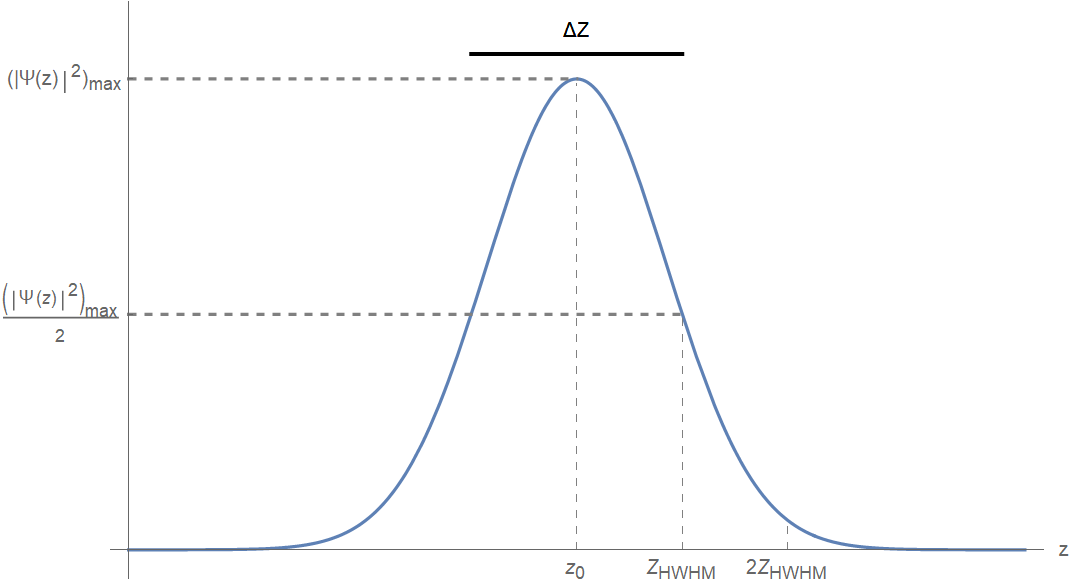
\includegraphics[width=0.9\textwidth]{atom_wave_func_pos_space.png}
\caption{Atomic wave function in position space. The wave packet is centered about $z_{0}$ and has a width equal to $2Z_{HWHM}$ where $Z_{HWHM}$ defines the half width at half maximum of the distribution function.}
\label{atom_wave_func_pos_space}
\end{figure}

Next, we consider the wave function of the atom in position space to be a gaussian like wave packet, initially centered at $z_{0}$. We already worked out the evolution of such wave packet in the last section. We re-write here the time evolution of the free wave packet

\begin{multline}\label{atom_wave_function_position_space}
    \Psi (z, t) = \left[\frac{1}{2 \pi \big(\sigma_{z}(t)\big)^2} \right]^{1/4} \exp \left[-\frac{1}{4} \frac{ \big(z - z_{0} - \upsilon_{g} t \big)^{2}}{\big(\sigma_{z}(t)\big)^{2}} \right] \exp \left[-\frac{i}{2} \arctan\Bigg(\frac{\beta t }{\big(\sigma_{z}(0)\big)^{2}}\Bigg) \right] \\ \exp \left[i \bigg(k_{0}(z-z_{0}) - w_{0}t + \frac{ \beta t (z - z_{0} - \upsilon_{g} t)^{2}}{ 4[\sigma_{z}(t)\sigma_{z}(0)]^{2}} \bigg) \right].
\end{multline}

Therefore, the initial wave packet will be given by

\begin{equation}\label{initial_atom_wave_function_position_space}
    \Psi (z, 0) = \left[\frac{1}{2 \pi \big(\sigma_{z}(0)\big)^2} \right]^{1/4} \exp \left[-\frac{1}{4}\bigg(\frac{z-z_{0}}{\sigma_{z}(0)}\bigg)^{2} \right] \exp \left[i \bigg(k_{0}(z-z_{0})\bigg) \right],
\end{equation}

where $\sigma_{z}(0)$ is the initial standard deviation of the distribution defined in the Eq. \ref{free_wave_packet_width}.

The complex modulus of this wave packet is a distribution for the probability of finding the atom in position space, i.e.,

\begin{equation}\label{initial_atom_wave_function_position_space_probability_distribution}
    |\Psi (z, 0)|^{2} = \frac{1}{\sigma_{z}(0) \sqrt{2 \pi}} \exp \left[-\frac{1}{2}\bigg(\frac{z-z_{0}}{\sigma_{z}(0)}\bigg)^{2} \right].
\end{equation}

We can define the half width at half maximum of this distribution and name the value of the independent variable $z$ at this point as $Z_{HWHM}$. In the Fig. \ref{atom_wave_func_pos_space}, we can see the initial atomic probability distribution in position space (Eq. \ref{initial_atom_wave_function_position_space_probability_distribution}). Notice that we have defined the width of the atomic wave function as follows.

\begin{equation}
  \Delta Z = 2|Z_{HWHM} - z_{0}|.
\end{equation}

It can be easily shown that the full with at half maximum for the normal distribution is given by

\begin{equation}\label{FWHM_normal_distribution}
Z_{FWHM} = 2\sqrt{2ln2} \sigma_{z}(0) = 2 Z_{HWHM}
\end{equation}

We will choose to use a coordinate system such that $z_{0}=0$. Thus, we can write

\begin{equation}\label{width_zhwhm}
  \Delta Z = 2Z_{HWHM} = Z_{FWHM}.
\end{equation}

Now, if we evaluate the detuning at $z = 2Z_{HWHM}$, we get

\begin{equation}
  \delta (2Z_{HWHM}) = 2\frac{\mu_{B} g_{F} m_{F} \eta}{\hbar} Z_{HWHM}
\end{equation}

i.e.,

\begin{equation}\label{position_at_zhwhm}
  2Z_{HWHM} = \delta (2Z_{HWHM}) \frac{\hbar}{\mu_{B} g_{F} m_{F} \eta}.
\end{equation}

Thereby, to determine the width of our atom's wave function, we just need to determine the detuning at $z = Z_{HWHM}$. In order to do so, firstly, we recall that the probability of finding the atom in the excited state at time $t$ when it was initially in the ground state at $t=0$ is given by

\begin{equation}\label{rabi_oscillations_exact}
  |c_{e}(t)|^{2} =\frac{\Omega^{2}}{\tilde{\Omega}^{2}} \sin^{2}\bigg[\frac{\tilde{\Omega} t}{2} \bigg],
\end{equation}

where $\tilde{\Omega}$ is defined in terms of the Rabi flopping frequency $\Omega$ and the detuning $\delta$, i.e.,

\begin{equation}
  \tilde{\Omega} = \sqrt{\delta^{2} + \Omega^{2}}.
\end{equation}

Now, a physical argument comes into play. We need to evaluate the detuning at $2z_{HWHM}$. In order to do so, we will suppose that the detuning evaluated at $2z_{HWHM}$ is such that the probability of transition at this position  is zero, i.e.,

\begin{equation}\label{detuning_condition}
\sqrt{\big[ \delta (2z_{HWHM}) \big]^{2} + \Omega^{2}} \bigg( \frac{t}{2} \bigg) = \pi.
\end{equation}

Furthermore, we will take the probability of transition for positions $|z| \ge 2 Z_{HWHM}$ to be zero, i.e,

\begin{equation}\label{position_condition}
|c_{e}(t)|^{2} =
    \begin{cases}
        \frac{\Omega^{2}}{\tilde{\Omega}^{2}} \sin^{2}\bigg[\frac{\tilde{\Omega} t}{2} \bigg] & \text{if } |z| < 2 Z_{HWHM}\\
        0 & \text{if } |z| \ge 2 Z_{HWHM}
    \end{cases}
\end{equation}

The Eqs. \ref{detuning_condition} and \ref{position_condition} constitute the conditions of our approximation. This approximation makes sense because the detuning evaluated at positions farther away from the position that defines the width of the atom ($z=2Z_{HWHM}$) should be such that the probability of transition is always zero. In other words, we cannot induce transitions in the atom if the perturbation is applied in a position where the probability of finding the atom is zero.

We can write down a function that approximately satisfies the conditions in the Eqs. \ref{detuning_condition} and \ref{position_condition}. We will use one more time the gaussian distribution, but this time the independent variable will be the detuning. We will define as before the full width at half maximum of this distribution

\begin{equation}\label{FWHM_normal_distribution}
\delta_{FWHM} = 2\sqrt{2ln2} \sigma_{\delta}(0)
\end{equation},

where $\sigma_{\delta}(0)$ is the standard deviation of the distribution.
Therefore,

\begin{equation}\label{rabi_oscillations_approx}
  |c_{e}(t)|^{2} \equiv f(\delta) = \frac{1}{f (0)} \frac{1}{\sigma_{\delta}(0) \sqrt{2 \pi}} \exp \left[-\frac{1}{2}\bigg(\frac{\delta-\delta_{0}}{\sigma_{\delta}(0)}\bigg)^{2} \right],
\end{equation}

where we have normalized the distribution such that the probability of transition when $\delta = 0$ equals $1$ for all times, i.e., $f(0)=1$. Finally, we choose the standard deviation to be equal to the detuning evaluated at  $z=2Z_{HWHM}$, i.e.,

\begin{equation}
    \sigma_{\delta}(0) = \delta(2Z_{HWHM})
\end{equation}

This approximation and the exact form of the transition probability versus the detuning can be seen in the Fig. \ref{ce2_VS_detuning}.

\begin{figure}
    \centering
    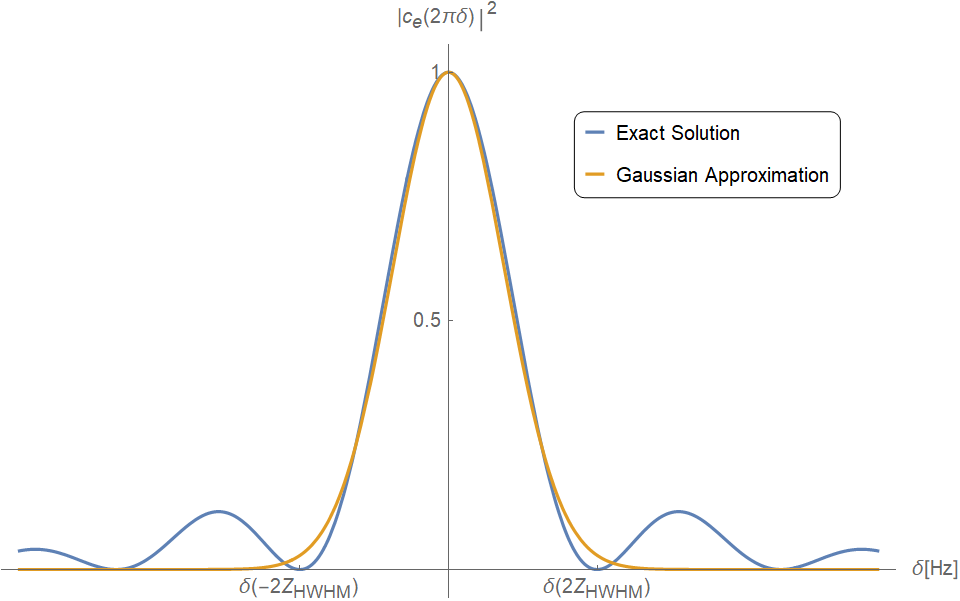
\includegraphics[width=0.9\textwidth]{ce2_VS_detuning_general.png}
     \caption{Probability of transition for the atom due to Rabi oscillations from the ground state to the excited state versus the detuning ($\Omega t$ is maintained fixed). The exact solution corresponds to the Eq. \ref{rabi_oscillations_exact} while the gaussian approximation corresponds to the Eq. \ref{rabi_oscillations_approx}. This gaussian function approximately satisfies the conditions used to estimate the detuning at $z=2Z_{HWHM}$ (Eqs. \ref{detuning_condition} and \ref{position_condition}).}
     \label{ce2_VS_detuning}
\end{figure}

Returning to our original problem, we can use the Eq. \ref{detuning_condition} to determine the detuning at $z=2Z_{HWHM}$, i.e.,

\begin{equation}\label{detuning_at_zhwm}
\delta (2z_{HWHM}) = \frac{\sqrt{4 \pi^{2} - \Omega^{2} t^{2}}}{t}.
\end{equation}

Thus, the width of the atom's wave function can be computed using Eqs. \ref{width_zhwhm}, \ref{position_at_zhwhm}, and \ref{detuning_at_zhwm}, i.e.,

\begin{equation}
\Delta Z = \frac{\sqrt{4 \pi^{2} - \Omega^{2} t^{2}}}{t} \frac{\hbar}{\mu_{B} g_{F} m_{F} \eta}.
\end{equation}

Thereby, we can use $\Omega$ and $t$ to control the width of the atom's wave function. For experimental purposes, we would like to have $\Omega$ fixed. Therefore, we can use $t$ to prepare the initial width. Specifically, if we use a $\pi$-pulse, i.e., $t=\pi/\Omega$. Then, the initial width will be given by

\begin{equation}
\Delta Z = \sqrt{3} \Omega \frac{\hbar}{\mu_{B} g_{F} m_{F} \eta}.
\end{equation}

Finally, we remember that in the case of light pulses, the electric field dominates and the Rabi flopping frequency is usually taken to be

\begin{equation*}
\Omega = \frac{- e \textbf{E} \cdot \bra{e} \textbf{r} \ket{g}}{\hbar},
\end{equation*}

where $\textbf{r}$ is the position operator, $\textbf{E}$ is the electric field, and $e$ is the electron charge. Nonetheless, in the case of the hyperfine levels that we are considering (Eq. \ref{hyperfine_levels}), the matrix elements of the position operator vanish  \cite{Steck2010}. Therefore, the Rabi flopping frequency will depend solely on the magnetic field, i.e.,

\begin{equation}
\Omega = \frac{- \textbf{B} \cdot \bra{e} \boldsymbol{\mu} \ket{g}}{\hbar},
\end{equation}

\subsection{Initial Atomic Cloud Preparation}
In the last section, we showed how to estimate the initial atomic width of the alkali atoms to be used during the interferometry process. In this section, we will use those results to show how we can prepare an atomic cloud sample of alkali atoms with a definite width and estimate within which time range our estimation is a good approximation.

\bibliographystyle{plain}
\bibliography{cites.bib}

























\begin{comment}
\section{Some examples to get started}

Your introduction goes here! Simply start writing your document and use the Recompile button to view the updated PDF preview. Examples of commonly used commands and features are listed below, to help you get started.

Once you're familiar with the editor, you can find various project setting in the Overleaf menu, accessed via the button in the very top left of the editor. To view tutorials, user guides, and further documentation, please visit our \href{https://www.overleaf.com/learn}{help library}, or head to our plans page to \href{https://www.overleaf.com/user/subscription/plans}{choose your plan}.

\subsection{How to create Sections and Subsections}

Simply use the section and subsection commands, as in this example document! With Overleaf, all the formatting and numbering is handled automatically according to the template you've chosen. If you're using Rich Text mode, you can also create new section and subsections via the buttons in the editor toolbar.

\subsection{How to include Figures}

First you have to upload the image file from your computer using the upload link in the file-tree menu. Then use the include graphics command to include it in your document. Use the figure environment and the caption command to add a number and a caption to your figure. See the code for Figure \ref{fig:frog} in this section for an example.

Note that your figure will automatically be placed in the most appropriate place for it, given the surrounding text and taking into account other figures or tables that may be close by. You can find out more about adding images to your documents in this help article on \href{https://www.overleaf.com/learn/how-to/Including_images_on_Overleaf}{including images on Overleaf}.

\begin{figure}
\centering
\includegraphics[width=0.3\textwidth]{frog.jpg}
\caption{\label{fig:frog}This frog was uploaded via the file-tree menu.}
\end{figure}

\subsection{How to add Tables}

Use the table and tabular environments for basic tables --- see Table~\ref{tab:widgets}, for example. For more information, please see this help article on \href{https://www.overleaf.com/learn/latex/tables}{tables}. 

\begin{table}
\centering
\begin{tabular}{l|r}
Item & Quantity \\\hline
Widgets & 42 \\
Gadgets & 13
\end{tabular}
\caption{\label{tab:widgets}An example table.}
\end{table}

\subsection{How to add Comments and Track Changes}

Comments can be added to your project by highlighting some text and clicking ``Add comment'' in the top right of the editor pane. To view existing comments, click on the Review menu in the toolbar above. To reply to a comment, click on the Reply button in the lower right corner of the comment. You can close the Review pane by clicking its name on the toolbar when you're done reviewing for the time being.

Track changes are available on all our \href{https://www.overleaf.com/user/subscription/plans}{premium plans}, and can be toggled on or off using the option at the top of the Review pane. Track changes allow you to keep track of every change made to the document, along with the person making the change. 

\subsection{How to add Lists}

You can make lists with automatic numbering \dots

\begin{enumerate}
\item Like this,
\item and like this.
\end{enumerate}
\dots or bullet points \dots
\begin{itemize}
\item Like this,
\item and like this.
\end{itemize}

\subsection{How to write Mathematics}

\LaTeX{} is great at typesetting mathematics. Let $X_1, X_2, \ldots, X_n$ be a sequence of independent and identically distributed random variables with $\text{E}[X_i] = \mu$ and $\text{Var}[X_i] = \sigma^2 < \infty$, and let
\[S_n = \frac{X_1 + X_2 + \cdots + X_n}{n}
      = \frac{1}{n}\sum_{i}^{n} X_i\]
denote their mean. Then as $n$ approaches infinity, the random variables $\sqrt{n}(S_n - \mu)$ converge in distribution to a normal $\mathcal{N}(0, \sigma^2)$.


\subsection{How to change the margins and paper size}

Usually the template you're using will have the page margins and paper size set correctly for that use-case. For example, if you're using a journal article template provided by the journal publisher, that template will be formatted according to their requirements. In these cases, it's best not to alter the margins directly.

If however you're using a more general template, such as this one, and would like to alter the margins, a common way to do so is via the geometry package. You can find the geometry package loaded in the preamble at the top of this example file, and if you'd like to learn more about how to adjust the settings, please visit this help article on \href{https://www.overleaf.com/learn/latex/page_size_and_margins}{page size and margins}.

\subsection{How to change the document language and spell check settings}

Overleaf supports many different languages, including multiple different languages within one document. 

To configure the document language, simply edit the option provided to the babel package in the preamble at the top of this example project. To learn more about the different options, please visit this help article on \href{https://www.overleaf.com/learn/latex/International_language_support}{international language support}.

To change the spell check language, simply open the Overleaf menu at the top left of the editor window, scroll down to the spell check setting, and adjust accordingly.

\subsection{How to add Citations and a References List}

You can simply upload a \verb|.bib| file containing your BibTeX entries, created with a tool such as JabRef. You can then cite entries from it, like this: \cite{greenwade93}. Just remember to specify a bibliography style, as well as the filename of the \verb|.bib|. You can find a \href{https://www.overleaf.com/help/97-how-to-include-a-bibliography-using-bibtex}{video tutorial here} to learn more about BibTeX.

If you have an \href{https://www.overleaf.com/user/subscription/plans}{upgraded account}, you can also import your Mendeley or Zotero library directly as a \verb|.bib| file, via the upload menu in the file-tree.

\subsection{Good luck!}

We hope you find Overleaf useful, and do take a look at our \href{https://www.overleaf.com/learn}{help library} for more tutorials and user guides! Please also let us know if you have any feedback using the Contact Us link at the bottom of the Overleaf menu --- or use the contact form at \url{https://www.overleaf.com/contact}.

\bibliographystyle{alpha}
\bibliography{sample}

\end{comment}

\end{document}